\documentclass[11pt,oneside]{article}
\usepackage[T1]{fontenc}
\usepackage[utf8]{inputenc}
\usepackage{lmodern}
\usepackage[margin=1in,headheight=15pt]{geometry}
\usepackage{microtype}
\usepackage{amsmath,amssymb,amsthm,mathtools}
\usepackage{booktabs,longtable,tabularx,array}
\usepackage{enumitem}
\usepackage{xcolor}
\usepackage{listings}
\usepackage{fancyhdr}
\usepackage{hyperref}
\usepackage{url}
\usepackage{graphicx}
\usepackage{tikz}
\usetikzlibrary{arrows.meta,positioning,shapes.geometric,fit}

\definecolor{deepblue}{RGB}{28,62,104}
\definecolor{softblue}{RGB}{231,239,248}
\definecolor{softgray}{RGB}{245,246,248}
\definecolor{darkgreen}{RGB}{31,103,72}
\definecolor{darkred}{RGB}{145,47,47}
\hypersetup{colorlinks=true,linkcolor=deepblue,citecolor=darkgreen,urlcolor=deepblue,
  pdftitle={STRIVE-iPRA},pdfauthor={OpenAI}}

\pagestyle{fancy}
\fancyhf{}
\lhead{STRIVE-iPRA}
\rhead{Finite strategy-table realization in iPRA}
\cfoot{\thepage}

\setlist[itemize]{leftmargin=1.6em,itemsep=0.25em,topsep=0.35em}
\setlist[enumerate]{leftmargin=1.8em,itemsep=0.25em,topsep=0.35em}
\setlength{\parindent}{1.2em}
\setlength{\parskip}{0.15em}
\setcounter{tocdepth}{2}

\newtheorem{theorem}{Theorem}[section]
\newtheorem{lemma}[theorem]{Lemma}
\newtheorem{proposition}[theorem]{Proposition}
\newtheorem{corollary}[theorem]{Corollary}
\theoremstyle{definition}
\newtheorem{definition}[theorem]{Definition}
\newtheorem{example}[theorem]{Example}
\newtheorem{contract}[theorem]{Contract}
\theoremstyle{remark}
\newtheorem{remark}[theorem]{Remark}
\newtheorem{warning}[theorem]{Warning}

\newcommand{\N}{\mathbb N}
\newcommand{\ipra}{\mathrm{iPRA}}
\newcommand{\PRAAx}{\mathsf{PRAAx}}
\newcommand{\Prf}{\mathsf{Prf}}
\newcommand{\True}{\mathbf 1}
\newcommand{\False}{\mathbf 0}
\newcommand{\Val}{\mathsf{Val}}
\newcommand{\Chk}{\mathsf{Check}}
\newcommand{\Pos}{\mathsf{Pos}}
\newcommand{\Neg}{\mathsf{Neg}}
\newcommand{\pack}{\mathsf{pack}}
\newcommand{\digit}{\mathsf{digit}}
\newcommand{\pref}{\mathsf{pref}}
\newcommand{\Obs}{\mathsf{Obs}}
\newcommand{\Valid}{\mathsf{Valid}}
\newcommand{\Res}{\mathsf{Res}}
\newcommand{\Goal}{\mathsf{Goal}}
\newcommand{\code}[1]{\texttt{#1}}
\newcommand{\sequent}[3]{#1\;\vdash_{#2}\;#3}

\lstdefinestyle{lean}{
  basicstyle=\ttfamily\small,
  backgroundcolor=\color{softgray},
  frame=single,
  rulecolor=\color{gray!35},
  breaklines=true,
  columns=fullflexible,
  keepspaces=true,
  showstringspaces=false,
  keywordstyle=\color{deepblue}\bfseries,
  commentstyle=\color{darkgreen},
  stringstyle=\color{darkred}
}
\lstset{style=lean}

\begin{document}
\pagenumbering{gobble}

\begin{titlepage}
\centering
\vspace*{1.2cm}
{\Huge\bfseries STRIVE-iPRA\par}
\vspace{0.35cm}
{\LARGE Strategy-Table Realization with Interface Verification and Elimination\par}
\vspace{0.9cm}
{\large A kernel-facing framework for embedding finite mathematical interactions in intuitionistic primitive recursive arithmetic\par}
\vfill
\begin{tabular}{rl}
Repository baseline: & \code{VladimirReshetnikov/ProveIt} \\
Pinned commit: & \code{58627ed89814ba122e1f0f012f1aba103cda267b} \\
Date: & 16 November 2026 \\
Primary target: & \code{Prf PRAAx Gamma phi}
\end{tabular}
\vfill
{\small Research artifact prepared by OpenAI.  The mathematical arguments are
human-readable proofs.  The packet claims no new Lean-kernel-checked theorem;
formalization status is stated theorem by theorem.\par}
\end{titlepage}
\pagenumbering{roman}

\begin{abstract}
The ProveIt repository now contains a checked ordinary presentation of
intuitionistic primitive recursive arithmetic, an extensive arithmetic library,
open-sequent transport, and a large collection of research packets based on
finite certificates, demand propagation, traces, and stable observations.  The
remaining obstacle is not a lack of high-level ideas.  It is the gap between an
abstract statement such as ``store a strategy for every adversarial reply'' and
a concrete object-language term, checker, and derivation in
\(\Prf\;\PRAAx\;\Gamma\;\varphi\).

This report develops STRIVE-iPRA, a realization layer for that gap.  For each
\emph{fixed} bounded formula built from reflected primitive-recursive atoms,
conjunction, disjunction, and bounded quantifiers, a metalevel compiler produces
concrete primitive-recursive functions for its Boolean value, positive and
negative certificate bounds, canonical signed strategy codes, and certificate
checkers.  Variable-length tables are represented by one natural number using
heterogeneous mixed-radix notation.  Positive and negative certificates are
dual: a certificate chooses one child at nodes controlled by its side and
contains a table of certificates at nodes controlled by the other side.  We
prove, constructively and by finite structural specialization, that accepted
positive codes imply the formula, accepted negative codes imply its
intuitionistic negation, and the canonical code for the computed side is
accepted.

The strategy compiler is embedded in a broader boundary-aware framework.
Proof-local certificates are eliminated by existential elimination;
noncanonical certificates expose only exact, quotient, or metric-stable
observations; and a least code is named only when the public theorem actually
requires one.  Finite monotone demand closure converts cyclic precision
requirements into a clocked schedule.  Missing height bounds, moduli,
separation estimates, finite-cover certificates, or producer theorems are not
hidden: they remain exact residual formulas in an open \(\PRAAx\) sequent.
This discipline resolves many recurring formalization difficulties while
making clear which obstacles are genuinely theorem-specific.

The packet includes full human proofs, a tested Python reference implementation,
JSON fixtures, a no-placeholder structural Lean candidate, and
source-oriented Lean blueprints for the arithmetic and compiler layers.  Since
Lean was unavailable in the artifact runtime, no new kernel-checked result is
claimed.
\end{abstract}

\section*{Executive statement of the result}

Let \(A(\vec a)\) be a fixed formula generated by
\[
  R(\vec t),\qquad A\wedge B,\qquad A\vee B,
  \qquad \exists x<b(\vec a,\vec z)\,A,
  \qquad \forall x<b(\vec a,\vec z)\,A,
\]
where every bound and atomic test is represented by a fixed
primitive-recursive symbol and each atom has a checked reflection theorem.
STRIVE constructs primitive-recursive terms
\[
 \Val_A,\quad P_A^+,P_A^-,\quad C_A^+,C_A^-,
 \quad \kappa_A^+,\kappa_A^-
\]
and generates ordinary iPRA derivations of the following forms:
\begin{align*}
 &\Val_A\in\{0,1\},\\
 &\Val_A=1\;\leftrightarrow\;A,\\
 &C_A^+(\vec a,c)=1\;\longrightarrow\;A(\vec a),\\
 &C_A^-(\vec a,c)=1\;\longrightarrow\;\neg A(\vec a),\\
 &C_A^\pm(\vec a,c)=1\;\longrightarrow\;c<P_A^\pm(\vec a),\\
 &\Val_A=1\;\longrightarrow\;C_A^+(\vec a,\kappa_A^+)=1,\\
 &\Val_A=0\;\longrightarrow\;C_A^-(\vec a,\kappa_A^-)=1.
\end{align*}
The formula is fixed at code-generation time.  The object theory performs only
primitive recursion on numerical bounds and quantifier-free induction; it does
not evaluate arbitrary formula codes.

The principal new realization device is the exact code bound.  If a node
requires certificates for all children and the child code spaces have sizes
\(B_0,\ldots,B_{N-1}\), its table has the tight bound
\(\prod_{i<N}B_i\) and code
\[
  \sum_{i<N} c_i\prod_{j<i}B_j.
\]
If a node requires one child certificate, its disjoint-union space has bound
\(\sum_{i<N}B_i\), and the code is a prefix sum plus the selected child code.
These two operations exactly mirror universal and existential proof behavior.

\tableofcontents
\clearpage
\pagenumbering{arabic}
\section{Repository baseline and the actual formal target}

\subsection{Why another abstract calculus would be a mistake}

The central design decision is to use the repository's ordinary iPRA calculus
as the public interface.  In the pinned tree, primitive-recursive symbols are
generated by zero, successor, projections, composition, and primitive
recursion; terms are applications of those symbols to finitely scoped
variables; and \(\PRAAx\) consists of the defining equations, the successor
axioms, and induction for quantifier-free formulas.  Derivability is the
intuitionistic natural-deduction relation
\[
  \Prf\;\PRAAx\;\Gamma\;\varphi,
  \qquad\text{written in Lean as }\code{Gamma |- [PRAAx] phi}.
\]
The existing derivation library already proves substantial arithmetic in this
judgment.  The bridge transports closed and open sequents to the Foundation
presentation.  Consequently a new framework should compile into this judgment,
not ask downstream developments to adopt another proof system.

There are three different levels that must not be conflated.

\begin{enumerate}
\item A \emph{semantic metaprogram} is an ordinary Lean or Python function
which evaluates a finite object on the host natural numbers.  It is useful for
generating symbols and tests, but its correctness is not an iPRA theorem.
\item A \emph{proof-producing metacompiler} generates a finite Lean expression
whose type is a \(\Prf\;\PRAAx\) judgment.  The generator is untrusted; the
Lean kernel checks its output.
\item An \emph{object-language universal interpreter} is a primitive-recursive
program inside iPRA that consumes a code of an arbitrary formula or proof.
That is a much stronger and more cumbersome construction.  STRIVE does not
need it.
\end{enumerate}

The framework therefore specializes a fixed mathematical interface at the
metalevel.  If a theorem contains seven bounded quantifier nodes, the compiler
emits seven finite constructor applications.  The only object-level recursion
is over numerical bounds, traces, or table lengths.  This fixed-program
principle is what keeps every invariant quantifier-free.

\subsection{Checked infrastructure reused directly}

The formalization plan assumes the following existing components.

{\small\begin{longtable}{>{\raggedright\arraybackslash}p{0.34\textwidth}>{\raggedright\arraybackslash}p{0.58\textwidth}}
\toprule
Component & Role in STRIVE \\
\midrule
\endfirsthead
\toprule
Component & Role in STRIVE \\
\midrule
\endhead
\code{ConciseIPRA.PR} & Defines \code{PR}, \code{PTm}, \code{PRAAx},
instantiated defining equations, and quantifier-free induction. \\
\code{ConciseIPRA.Deduction} & Defines \code{Prf}; provides substitution,
weakening, simultaneous cut \code{Prf.trans}, and existential elimination. \\
\code{IPRADerivations.}\newline\code{Core.Basic} & Arithmetic notation, open induction helper,
instantiation of closed derivations, and congruence lemmas. \\
\code{Core.Order} and \code{Core.Semiring} & Decidable equality/order,
monotonicity, cancellation, and the finite interval algebra needed for code
bounds. \\
\code{Core.Powers} & Prefix powers in the uniform-base special case and the
algebra needed for product bounds. \\
\code{Core.MultiSums} & Primitive-recursive finite sums and products with
parameters, their defining equations, and bounded congruence. \\
\code{Core.Division} & Total quotient and remainder and uniqueness for positive
divisors. \\
\code{Core.Search} & Least bounded search with foundness and minimality
proofs. \\
\code{IPRABridge} & Closed and finite open-sequent transport to Foundation
iPRA after an ordinary derivation has been completed. \\
\bottomrule
\end{longtable}}

The use of these modules is not merely a software convenience.  It gives the
mathematical proof its intended strength.  For example, selecting the first
successful branch is not an appeal to an external choice function; it is an
application of an already formalized bounded-search recurrence.  Decoding one
digit is not an unverified use of machine division; it is reduced to the
object-theory existence and uniqueness equations for quotient and remainder.

\subsection{Status separation}

A recurring source of confusion in research packets is the phrase
``formalizable in iPRA.''  It may mean any of the following:

\begin{itemize}
\item the mathematical argument is finitary;
\item a host-language program has been tested;
\item Lean definitions have been written but contain placeholders;
\item a Lean theorem about \(\N\) has been proved;
\item an actual \(\Prf\;\PRAAx\) derivation has been checked;
\item that derivation has additionally been exported to a second presentation.
\end{itemize}

STRIVE records these statuses separately.  The present report supplies complete
human proofs and executable finite tests.  The small structural kernel is a
no-placeholder source candidate.  The arithmetic and compiler modules expose
all unfinished proof obligations as visible \code{sorry} milestones.  No new
kernel-checked theorem is asserted.

\subsection{The main unresolved engineering boundary}

Earlier framework packets already explain how to use finite queries, traces,
backward viability, stable observations, and residual producer assumptions.
Their most persistent unformalized step is a phrase of the form

\begin{quote}
At a universally controlled node, store a certificate for every response; at
an existentially controlled node, store one successful response.
\end{quote}

For a paper proof this is enough.  For \(\PRAAx\), four additional questions
must be answered.

\begin{enumerate}
\item What is the primitive-recursive bound on the whole certificate code?
\item How is a variable-length table represented by one natural number?
\item How does the checker recover the \(i\)-th subcertificate with equations
available in the object theory?
\item Which quantifier-free invariant proves that the checker has inspected
all required entries?
\end{enumerate}

The mixed-radix and signed-compiler layers below answer these questions in a
form designed around the repository's current arithmetic API.

\section{The STRIVE architecture}

\subsection{Finite observations as the common language}

Many mathematical objects are infinitary when presented extensionally: a real
number has arbitrarily accurate rational approximations, a continuous function
has values at infinitely many inputs, an algebraic branch has infinitely many
compatible truncations, and a model or strategy may respond to every possible
challenge.  A finite proof does not consume the entire object.  It asks finitely
many questions and uses finitely many answers.

STRIVE represents a concept by a \emph{finite observation interface}.  For an
input parameter \(a\), a query \(q\), and a certificate \(c\), the interface
contains primitive-recursive data
\[
 B(a,q),\qquad C(a,q,c)\in\{0,1\},\qquad O(a,q,c),
\]
where \(c<B(a,q)\) is the declared finite code range, \(C=1\) means that the
certificate answers the query correctly, and \(O\) is the part of the answer
visible to the consumer.  The producer contract is a formula such as
\[
  \forall q<Q(a)\;\exists c<B(a,q)\; C(a,q,c)=1.
\]
A theorem-specific proof may establish this contract outright.  If it cannot,
the contract remains an explicit residual hypothesis.

This interface covers several familiar situations.

\begin{itemize}
\item For an exact finite object, \(q\) may be trivial and \(O=c\).
\item For a real number, \(q\) is a requested precision and \(O\) is a rational
interval or approximation.
\item For a root of a polynomial, \(c\) may contain a box and a local
verification trace, while \(O\) is a symmetric polynomial of all roots in the
box.
\item For a bounded game, \(q\) identifies a node and \(c\) is a signed
strategy code.
\item For a finite cover, \(c\) identifies a covering patch and carries a
local estimate.
\end{itemize}

The important point is that the public theorem need not expose \(c\).  The
scope of a certificate is a design choice, formalized in Section~8.

\subsection{Five layers and their proof obligations}

The framework has five layers.

\begin{description}[leftmargin=2.3cm,style=nextline]
\item[Arithmetic layer]
Natural-number coding, bounded sums/products, quotient/remainder, pairing,
order, and least search.  This is mostly inherited checked infrastructure.

\item[Strategy layer]
A compiler from each fixed bounded formula to a Boolean value, two code spaces,
two checkers, and canonical signed codes.  Mixed-radix tables are the key new
realization device.

\item[Interaction layer]
A finite query graph or clocked state machine.  It computes the set of demanded
observations, verifies compatible transitions, and replays a successful finite
interaction.  Monotone cyclic demands are first closed on a finite product of
chains.

\item[Observation layer]
Rules for erasing noncanonical certificates.  Exact observers are independent
of the certificate, quotient observers are equivalent, and metric observers
have a bounded diameter.

\item[Boundary layer]
All theorem-specific inputs are formulas in an open \(\PRAAx\) context.  A
compiled theorem has the literal shape
\[
  R_1,\ldots,R_s,\Gamma\;\vdash_{\PRAAx}\;\Phi.
\]
Supplying derivations of the residuals closes the theorem by simultaneous cut.
\end{description}

\begin{center}
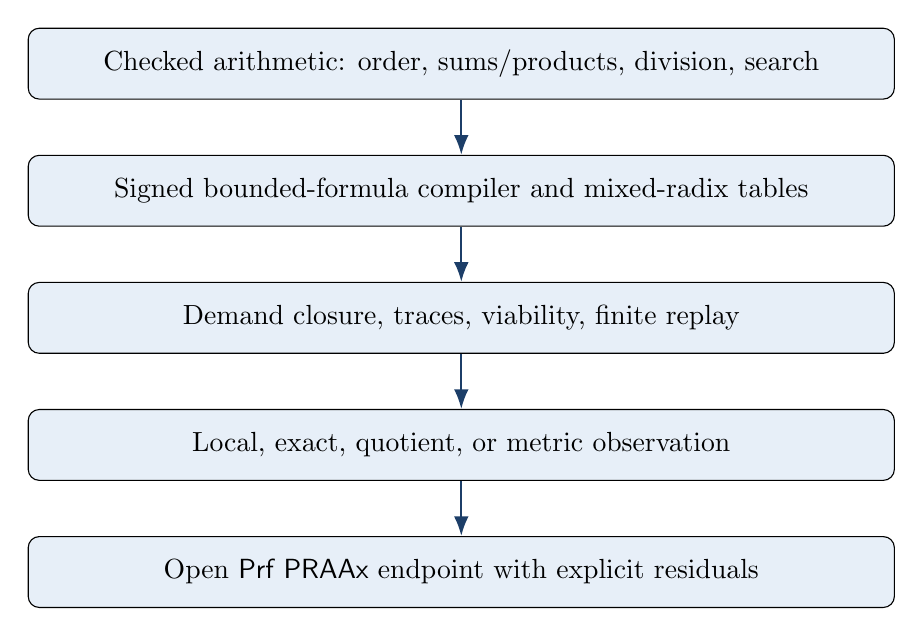
\begin{tikzpicture}[
  node distance=7mm,
  box/.style={draw,rounded corners,minimum width=11cm,minimum height=9mm,
    align=center,fill=softblue},
  arr/.style={-{Latex[length=2.5mm]},thick,deepblue}]
\node[box] (arith) {Checked arithmetic: order, sums/products, division, search};
\node[box,below=of arith] (strategy) {Signed bounded-formula compiler and mixed-radix tables};
\node[box,below=of strategy] (interaction) {Demand closure, traces, viability, finite replay};
\node[box,below=of interaction] (observer) {Local, exact, quotient, or metric observation};
\node[box,below=of observer] (boundary) {Open \(\Prf\;\PRAAx\) endpoint with explicit residuals};
\draw[arr] (arith) -- (strategy);
\draw[arr] (strategy) -- (interaction);
\draw[arr] (interaction) -- (observer);
\draw[arr] (observer) -- (boundary);
\end{tikzpicture}
\end{center}

\subsection{Two kinds of compilation}

The word ``compiler'' is used in two related senses.

First, the \emph{formula compiler} is structural.  Given a fixed bounded
formula, it constructs the value and signed-certificate package.  Its
metatheoretic recursion follows the syntax tree.

Second, the \emph{contract compiler} is graph based.  Given finitely many local
lemmas and data dependencies, it determines which queries are demanded,
instantiates local results, and composes their derivations.  Its object-level
work is a clocked recurrence or a finite sequence of cuts.

The two compilers meet at a simple interface: every local finite claim can be
turned into a Boolean reflected atom or a bounded formula, and every unresolved
local producer is retained as a boundary formula.  This separation prevents a
large monolithic universal checker.  It also lets arithmetic lemmas be checked
and reused independently of any particular application.

\subsection{Why signed certificates are preferable to truth values alone}

A Boolean evaluator answers whether a finite statement is true.  A proof
compiler needs more.

\begin{itemize}
\item When the value is one, it needs enough information to introduce every
existential and disjunction and to answer every universal or conjunction
challenge.
\item When the value is zero, it needs enough information to prove an
intuitionistic negation.  A bare zero is not a proof of failure; a
counterstrategy is.
\item For diagnosis, a negative certificate identifies a least failing query or
contains a table closing every attempted witness.
\item For composition, the checker can consume an externally supplied
certificate without trusting the producer that constructed it.
\end{itemize}

The positive and negative code spaces are therefore first-class and generally
have different sizes.  Their recurrences are not implementation accidents;
they are the numerical reflection of intuitionistic introduction and
elimination behavior.

\section{Boundary-aware contracts and proof composition}

\subsection{Open sequents are the correct output format}

A framework theorem should not silently assume that every mathematical
producer is available.  Suppose a finite argument needs a height bound, a
finite cover, a local root-separation estimate, and an arithmetic lemma.  The
right endpoint is
\[
  H(a),\;K(a),\;S(a),\;\Gamma(a)
  \;\vdash_{\PRAAx}\;\Phi(a),
\]
not a closed theorem whose prose says that these inputs are ``standard.''  Each
boundary is an ordinary formula in the same finite variable scope as the goal.
The existing structural rule \(\Prf.\mathsf{trans}\) then replaces every
boundary by a derivation of it.

\begin{theorem}[Boundary composition]
Let \(\Gamma=[B_1,\ldots,B_r]\) and suppose
\(\Gamma\vdash_{\PRAAx}A\).  If a context \(\Delta\) derives each
\(B_i\), then \(\Delta\vdash_{\PRAAx}A\).
\end{theorem}

\begin{proof}
The natural-deduction derivation may use a hypothesis rule at any occurrence of
some \(B_i\).  Simultaneous cut replaces that occurrence by the supplied
derivation.  Formally this is exactly the checked theorem
\(h.\mathsf{trans}(\mathsf{supply})\).  It is proved in the repository by
induction over the hypothesis list, repeatedly introducing an implication and
applying modus ponens.  No classical principle is involved.
\end{proof}

This theorem gives contract graphs a simple semantics.  A node is not a new
logical connective.  It is an ordinary derivation under a list of formulas.
Graph composition is simultaneous cut; parameter instantiation is
\(\Prf.\mathsf{subst}\); and graph reuse under more assumptions is weakening.

\subsection{Proof-local certificates}

The most common certificate should never cross a public boundary.  Let
\(V(\vec a,c)\) mean that \(c\) is a valid certificate and suppose the consumer
has a derivation
\[
 V(\vec a,c),\;\Gamma(\vec a)
 \;\vdash_{\PRAAx}\; A(\vec a),
\]
where the goal does not contain the bound certificate variable.  If the
producer proves
\[
 \Gamma(\vec a)\;\vdash_{\PRAAx}\;\exists c\,V(\vec a,c),
\]
then existential elimination gives \(\Gamma\vdash A\).

\begin{theorem}[Local certificate sealing]
A proof-local certificate requires neither a canonical choice nor a least
search.  Existential production and a certificate-parametric consumer suffice.
\end{theorem}

\begin{proof}
Open the producer's existential with a fresh variable \(c\), apply the consumer,
and close the existential elimination.  The eigenvariable condition is exactly
that \(A\) and the outer context are shifted from the smaller scope and hence do
not mention \(c\).  This is the checked \(\Prf.\mathsf{exE}\) rule.
\end{proof}

This observation removes a great deal of unnecessary canonicalization.  A
proof that merely needs a local path, basis, chart, root box, or finite cover
may consume whichever valid certificate the producer supplies.

\subsection{Exact residuals}

If the producer is not known, the same consumer gives the conditional theorem
\[
 \Gamma\vdash_{\PRAAx}
   (\exists c\,V(\vec a,c))\to A(\vec a).
\]
This formula is an \emph{exact residual}: it states precisely what remains to
be proved, in the object language and at the correct scope.  Exact residuals
are preferable to labels such as ``compactness'' or ``effective finiteness.''
They reveal whether the missing input is

\begin{itemize}
\item a numerical bound;
\item a finite list or table satisfying a checker;
\item a local implication used at each index;
\item a modulus mapping requested output precision to input precision;
\item a separation or lower-bound estimate;
\item or an actual unbounded theorem.
\end{itemize}

The distinction matters.  A checker for a proposed height bound may be fully
formalized even when no theorem produces such a bound in general.  The
framework can therefore finish the verifier and every downstream consequence
without pretending to solve the producer theorem.

\subsection{Contract normal form}

For practical composition, normalize every local component to the following
shape.

\begin{contract}[Finite contract node]
A node with parameters \(\vec a\) consists of:
\begin{enumerate}
\item a finite list of prerequisite formulas \(R_1(\vec a),\ldots,R_s(\vec a)\);
\item a bounded certificate predicate \(C(\vec a,c)=1\), optionally with an
explicit code bound \(c<B(\vec a)\);
\item a local derivation from the prerequisites and certificate validity to a
postcondition \(P(\vec a,c)\);
\item an escape declaration saying whether \(c\) is local, observed, or named.
\end{enumerate}
\end{contract}

A node with no certificate is the special case \(B=1\) and \(c=0\).  A node
with a table certificate uses the mixed-radix layer.  A node with an unresolved
producer includes \(\exists c<B\,C=1\) among its residuals.

\subsection{Acyclic composition}

If the dependency graph is acyclic, order its nodes topologically.  Start with
the derivation of the final node under all residuals.  Replace each internal
postcondition assumption by the derivation exported from its producer node.
Proof-local certificates are sealed as soon as the last consumer in their
scope has been processed.  The result is one ordinary open sequent under only
external residuals.

There is no need to internalize the graph structure in iPRA.  The graph is
metalevel compilation data.  The generated proof term is a finite nest of
\(\mathsf{trans}\), substitution, implication, and existential-elimination
steps.  Cyclic numerical demand dependencies are handled separately by finite
closure and a clock, not by circular proof terms.

\subsection{Scope discipline}

Several subtle errors are prevented by requiring a scope annotation on every
contract.

\begin{enumerate}
\item A certificate variable opened by existential elimination is fresh and
cannot occur in the outer goal.
\item A quantified body lives in scope \(n+1\), while its bound lives in scope
\(n\).  Substitution uses the repository's \(\mathsf{inst}\) and
\(\mathsf{shift}\) operations rather than informal renaming.
\item A formula transported through the Foundation bridge is first proved in a
common finite ConciseIPRA scope.  Distinct free variables are not collapsed by
an accidental assignment.
\item A metalevel callback is never inserted as though it were a \(PR\) symbol.
Every generated evaluator, bound, and checker has a concrete primitive-
recursive definition.
\end{enumerate}

The supplied \code{Kernel.lean} packages the first layer of this discipline in
small source-compatible declarations.  The larger compiler must preserve the
same explicit scoping throughout.

\section{Heterogeneous mixed-radix tables}

\subsection{Why one natural number is enough}

At a universal node a certificate may need one subcertificate for every
\(i<N\).  The number of entries depends on the input, and the bound on the
\(i\)-th subcertificate may depend on earlier quantified values.  A fixed tuple
type is therefore inadequate, while an abstract list would require a separate
list theory and coding layer.

Natural numbers already provide the needed finite container.  Let
\(B_0,\ldots,B_{N-1}\) be positive radices and let
\(0\le c_i<B_i\).  Define prefix products and the code by
\[
  P_0=1,\qquad P_{i+1}=P_iB_i,
  \qquad
  \pack_N(\vec c)=\sum_{i<N}c_iP_i.
\]
The total code range is \(0\le\pack_N(\vec c)<P_N\).  The \(i\)-th digit is
recovered by
\[
  \digit_i(x)=\bigl(\lfloor x/P_i\rfloor\bmod B_i\bigr).
\]
All operations are primitive recursive when \(N\), the digit function, and the
radix function are primitive recursive.  In the repository they are assembled
from bounded sums, bounded products, quotient, and remainder.

\subsection{The interval lemma}

The basic estimate is elementary but central.

\begin{lemma}[Append interval]
If \(0\le x<P\), \(0\le d<B\), and \(P,B>0\), then
\[
  0\le x+dP<PB.
\]
\end{lemma}

\begin{proof}
The lower bound is immediate.  Since \(d<B\), natural-number discreteness gives
\(d+1\le B\).  Therefore
\[
  x+dP < P+dP=(d+1)P\le BP.
\]
Every step is an order or semiring identity already available in ordinary iPRA.
The proof uses no subtraction by an unknown sign and no classical case split.
\end{proof}

\begin{theorem}[Packed-code bound]
Assume \(B_i>0\) and \(c_i<B_i\) for every \(i<N\).  Then
\[
  \pack_N(\vec c)<P_N.
\]
\end{theorem}

\begin{proof}
Use induction on \(N\).  For \(N=0\), the empty sum is zero and the empty
product is one.  In the successor step,
\[
 \pack_{N+1}=\pack_N+c_NP_N,
 \qquad P_{N+1}=P_NB_N.
\]
The induction hypothesis gives \(\pack_N<P_N\), and the append interval lemma
with \(x=\pack_N\), \(P=P_N\), \(d=c_N\), and \(B=B_N\) gives the result.  The
induction predicate is an inequality between primitive-recursive terms and is
quantifier-free.
\end{proof}

\subsection{Digit recovery}

Fix \(i<N\).  Split the packed sum into lower, current, and upper pieces:
\[
  \pack_N=L_i+c_iP_i+P_{i+1}U_i,
\]
where
\[
  L_i=\sum_{j<i}c_jP_j,
  \qquad
  U_i=\sum_{i<j<N}c_j\prod_{i<k<j}B_k.
\]
By the packed-code bound applied to the prefix, \(L_i<P_i\).  Since
\(P_{i+1}=P_iB_i\), we may rewrite
\[
 \pack_N=P_i(c_i+B_iU_i)+L_i.
\]
Division uniqueness for the positive divisor \(P_i\) therefore gives
\[
  \left\lfloor\frac{\pack_N}{P_i}\right\rfloor=c_i+B_iU_i,
  \qquad
  \pack_N\bmod P_i=L_i.
\]
A second use of division uniqueness, now for divisor \(B_i\), gives remainder
\(c_i\).  Thus \(\digit_i(\pack_N)=c_i\).

\begin{theorem}[Mixed-radix decoding]
Under the hypotheses of the packed-code bound, every \(i<N\) satisfies
\[
  \digit_i(\pack_N(\vec c))=c_i.
\]
\end{theorem}

\begin{proof}
The preceding calculation is the mathematical proof.  For a direct iPRA
formalization it is convenient to avoid defining \(U_i\) first.  Prove by
induction on \(N\) two lemmas simultaneously.

\begin{enumerate}
\item The newest digit of \(x+dP_N\) is \(d\) whenever \(x<P_N\) and
\(d<B_N\).
\item Appending \(dP_N\) leaves every earlier digit unchanged.
\end{enumerate}

For the newest digit, division uniqueness by \(P_N\) identifies quotient
\(d\) and remainder \(x\), and division by \(B_N\) identifies the remainder of
\(d\) as \(d\).  For an earlier index \(i<N\), \(P_N\) is divisible by
\(P_iB_i\); adding a multiple of \(P_iB_i\) changes the quotient by a multiple
of \(B_i\) and hence does not change its remainder modulo \(B_i\).  The
repository's finite-product recurrence supplies the factorization of prefix
products.  Applying the induction hypothesis to the old prefix completes the
proof.
\end{proof}

\subsection{Uniqueness and extensionality}

\begin{corollary}[Code extensionality]
If \(c_i,d_i<B_i\) for all \(i<N\), then
\[
  \pack_N(\vec c)=\pack_N(\vec d)
  \quad\Longleftrightarrow\quad
  \forall i<N\;c_i=d_i.
\]
\end{corollary}

\begin{proof}
The reverse implication follows from bounded-sum congruence.  For the forward
implication, apply \(\digit_i\) to both sides and use the decoding theorem.  In
the object proof, ``for all \(i<N\)'' is represented by a Boolean fold or by a
universally quantified implication whose matrix is quantifier-free; the
compiler chooses the form appropriate to the consumer.
\end{proof}

\subsection{Disjoint sums for one selected child}

Tables encode a certificate for every child.  A node controlled by the winning
side needs only one child.  Let child code space \(i\) have size \(B_i\), which
may be zero when no certificate of the requested sign can exist.  Define prefix
sums
\[
  S_0=0,
  \qquad S_{i+1}=S_i+B_i.
\]
The disjoint union has bound \(S_N\).  A pair \((i,c)
equation\) with
\(i<N\) and \(c<B_i\) is encoded as
\[
  S_i+c.
\]
Conversely, for every \(x<S_N\), the least \(i<N\) satisfying
\(x<S_{i+1}\) exists; minimality gives \(S_i\le x\), and
\(c=x\mathbin{\dot{-}}S_i<B_i\).  The owner index is computed by bounded
least search.  This is a particularly clean use of the existing
\code{Core.Search}: it supplies both foundness and minimality.

\begin{lemma}[Disjoint decoding]
For \(i<N\) and \(c<B_i\), the least owner of \(S_i+c\) is \(i\), and the local
code is \(c\).
\end{lemma}

\begin{proof}
For every \(j<i\), monotonicity of prefix sums gives
\(S_{j+1}\le S_i\le S_i+c\), so no earlier interval contains the code.  At
\(i\), \(c<B_i\) gives \(S_i+c<S_i+B_i=S_{i+1}\).  Least-search minimality and
truncated-subtraction cancellation yield the local code equation.
\end{proof}

\subsection{Zero radices and empty tables}

A tight table bound \(\prod_{i<N}B_i\) can be zero.  This is correct: if one
required child has no certificate of the demanded sign, no table certificate
exists.  The checker first verifies \(c<\prod B_i\).  Under that assumption the
product is positive, hence every factor is positive, so quotient/remainder
lemmas may safely be used.  If the table is empty, the product is one and the
unique code is zero.

For an initial Lean implementation one may instead use padded radices
\(B_i+1\), reject the sentinel digit \(B_i\), and later optimize to the tight
bound.  STRIVE's reference implementation uses the tight representation, and
the formalization plan states the positivity obligations explicitly.

\subsection{Primitive-recursive realization}

Let \(b(i,p)\) and \(c(i,p)\) be concrete primitive-recursive terms.  Define
\[
 \pref(i,p)=\prod_{j<i}b(j,p),
 \qquad
 \pack(N,p)=\sum_{i<N}c(i,p)\pref(i,p).
\]
The current repository already supplies parameterized finite products and
sums.  Hence \(\pref\) and \(\pack\) are concrete \(PR\) symbols with zero and
successor equations.  Digit access is the term
\[
 \operatorname{rem}\bigl(
   \operatorname{quo}(x,\pref(i,p)),\;b(i,p)
 \bigr).
\]
The Lean blueprint \code{STRIVE/MixedRadix.lean} is organized precisely around
these existing equations.  No abstract sequence type, quotient type, or
universal decoding relation is required.

\section{Bounded formulas as signed finite games}

\subsection{Formula grammar}

Fix a finite formula schema with free parameter tuple \(\vec a\).  Its atoms
are reflected primitive-recursive relations.  The grammar is
\[
 A ::= R(\vec t)\mid A\wedge A\mid A\vee A
       \mid \exists x<b(\vec a,\vec z)\,A
       \mid \forall x<b(\vec a,\vec z)\,A.
\]
The bound may depend on parameters and variables chosen by earlier quantifiers,
but not on the variable it bounds.  The formula tree is fixed in the
metatheory.  All numerical bounds may vary with the input.

An atom is represented by a Boolean term \(r(\vec a)\in\{0,1\}\) and checked
derivations
\[
 r=1\to R,\qquad r=0\to\neg R.
\]
Equivalently one may supply \(r=1\leftrightarrow R\) together with Booleanity.
The negative direction is constructively available because the atom is
decidable.  Negation need not be pushed through the entire formula: the signed
compiler directly constructs a proof of \(\neg A\) from a negative strategy.

\subsection{Game reading}

Read a positive certificate as a strategy for the prover and a negative
certificate as a strategy for the refuter.

\begin{center}
\begin{tabular}{lll}
\toprule
Node & Positive certificate & Negative certificate \\
\midrule
Atom & recomputed true atom & recomputed false atom \\
\(A\wedge B\) & certificates for both & one failing conjunct \\
\(A\vee B\) & one successful disjunct & certificates for both \\
\(\exists x<b\,A_x\) & one witness and child certificate & table for every witness \\
\(\forall x<b\,A_x\) & table for every challenge & one counterexample and child certificate \\
\bottomrule
\end{tabular}
\end{center}

The table cases use heterogeneous mixed radix.  The one-child cases use
disjoint sums.  This duality is exactly the intuitionistic proof theory.  A
negative certificate for \(A\wedge B\) is not a proof of the classically
stronger formula \(\neg A\vee\neg B\) obtained by an unrestricted De Morgan
law; it explicitly contains the branch and a proof of that branch's negation.
Similarly, a negative certificate for a bounded existential explicitly
contains a refutation for every candidate.

\subsection{Value functions}

Define the Boolean value structurally:
\begin{align*}
 \Val_R &= r,\\
 \Val_{A\wedge B} &= \Val_A\cdot\Val_B,\\
 \Val_{A\vee B} &= \mathsf{or}(\Val_A,\Val_B),\\
 \Val_{\exists x<b A_x} &= \mathsf{any}_{x<b}\Val_{A_x},\\
 \Val_{\forall x<b A_x} &= \mathsf{all}_{x<b}\Val_{A_x}.
\end{align*}
Here \(\mathsf{all}\) is a finite product of normalized Booleans, and
\(\mathsf{any}\) may be defined as the sign of a finite sum or by a direct
primitive recursion.  Empty conventions are
\[
 \mathsf{any}_{x<0}=0,
 \qquad
 \mathsf{all}_{x<0}=1.
\]
Every value is primitive recursive, and Booleanity follows by structural
specialization and quantifier-free induction for the folds.

\subsection{Positive and negative code-space bounds}

Let \(P_A^+(\vec a)\) and \(P_A^-(\vec a)\) be the sizes of the syntactic
positive and negative code spaces.  The recurrences are
\begin{align*}
 P_R^+&=1,&P_R^-&=1,\\
 P_{A\wedge B}^+&=P_A^+P_B^+,&
 P_{A\wedge B}^-&=P_A^-+P_B^-,\\
 P_{A\vee B}^+&=P_A^++P_B^+,&
 P_{A\vee B}^-&=P_A^-P_B^-,\\
 P_{\exists x<b A_x}^+&=\sum_{x<b}P_{A_x}^+,&
 P_{\exists x<b A_x}^-&=\prod_{x<b}P_{A_x}^-,\\
 P_{\forall x<b A_x}^+&=\prod_{x<b}P_{A_x}^+,&
 P_{\forall x<b A_x}^-&=\sum_{x<b}P_{A_x}^-.
\end{align*}
A bound may be zero.  For example, the positive space of an empty existential
has size zero, while its negative space is the singleton empty table.  These
are exact bounds; they do not assert that every syntactically shaped code is
valid.

The sum/product pattern is the numerical form of the game duality.  One branch
is a disjoint sum; all branches are a Cartesian product encoded by mixed radix.
This observation provides a simple audit: if a constructor's code-bound
recurrence does not match its proof rule, the compiler is wrong.

\subsection{Checkers}

For each formula define primitive-recursive predicates
\[
 C_A^+(\vec a,c),\qquad C_A^-(\vec a,c)
\]
with values in \(\{0,1\}\).  Every checker first verifies
\(c<P_A^\pm(\vec a)\).

At an atom the only code is zero, and the checker recomputes the atomic Boolean.
At a product node, mixed-radix decoding produces the child codes and the
checker conjoins their checks.  At a disjoint node, prefix sums locate the owner
interval and the checker invokes the corresponding child.  At a bounded
quantifier, the same operations occur over a variable number of children;
the checker uses a finite Boolean fold.

The checker is intentionally independent of the canonical producer.  An
external algorithm may provide a different valid strategy.  Soundness trusts
only the checker equation, not the history of the code.

\subsection{Canonical codes}

The canonical producer follows the value.

\begin{itemize}
\item At a product node, recursively produce all child codes and pack them.
\item At a disjoint node, use bounded least search to find the least child with
the required value, recursively produce its code, and add the corresponding
prefix sum.
\item At an empty product, return zero.
\end{itemize}

There are two canonical terms \(\kappa_A^+\) and \(\kappa_A^-\), but only the
one matching \(\Val_A\) is required to be accepted.  Defining both as total
primitive-recursive functions avoids partial terms.  Their behavior on the
wrong side is irrelevant.

\subsection{Counterstrategy content}

A negative certificate is more informative than a proof of decidability.
For a formula
\[
 \forall q<Q\;\exists z<Z(q)\;\forall e<E(q,z)\;R(q,z,e),
\]
a positive certificate is a table assigning each \(q\) one \(z\) and, for
that \(z\), a table of atomic successes for all \(e\).  A negative certificate
chooses one \(q_0\) and contains, for every candidate \(z<Z(q_0)\), one
counterexample \(e_z\) with a negative atomic certificate.  This is exactly the
failure explanation practitioners want from a finite search.

No excluded-middle principle is hidden here.  The alternatives are computed by
finite primitive recursion over decidable atomic tests.  The object proof of
the winning side is generated together with the computation.

\section{The signed compiler theorem}

\subsection{Statement}

\begin{theorem}[STRIVE bounded-formula compilation]
For every fixed bounded formula \(A(\vec a)\) over reflected primitive-recursive
atoms, one can effectively construct primitive-recursive terms
\[
 \Val_A,\quad P_A^+,P_A^-,\quad C_A^+,C_A^-,
 \quad \kappa_A^+,\kappa_A^-
\]
and ordinary iPRA derivations of
\begin{align}
 &\Val_A=0\vee\Val_A=1, \tag{6.1}\\
 &\Val_A=1\leftrightarrow A, \tag{6.2}\\
 &C_A^+(\vec a,c)=1\to A, \tag{6.3}\\
 &C_A^-(\vec a,c)=1\to\neg A, \tag{6.4}\\
 &C_A^\pm(\vec a,c)=1\to c<P_A^\pm(\vec a), \tag{6.5}\\
 &\Val_A=1\to C_A^+(\vec a,\kappa_A^+)=1, \tag{6.6}\\
 &\Val_A=0\to C_A^-(\vec a,\kappa_A^-)=1. \tag{6.7}
\end{align}
All derivations are uniform in the free numerical parameters of this fixed
formula.  The construction does not provide an object-language evaluator for
arbitrary formula codes.
\end{theorem}

\subsection{Metatheoretic induction}

The proof is a structural induction on the fixed syntax tree.  This induction
is performed by the compiler, not inside iPRA.  At each node, the compiler
combines already generated child symbols and child derivations with a finite
library lemma.  The result is a concrete finite Lean term.

Object-level induction occurs only inside bounded folds and searches.  Its
invariants are equations and order comparisons of primitive-recursive terms,
so the \(\PRAAx\) quantifier-free induction scheme applies.

We now give every constructor in enough detail to determine the Lean proof.

\subsection{Atoms}

Let \(r\) be a Boolean term reflecting \(R\).  Set
\[
 \Val_R=r,
 \qquad P_R^+=P_R^-=1,
 \qquad \kappa_R^+=\kappa_R^-=0.
\]
Define
\[
 C_R^+(c)= [c=0]\,[r=1],
 \qquad
 C_R^-(c)= [c=0]\,[r=0].
\]
Booleanity is supplied by the atom package.  The value equivalence is the
reflection theorem.  Positive and negative checker soundness are immediate,
and both canonical acceptance theorems reduce to reflexivity and the relevant
value hypothesis.

\subsection{Conjunction}

Assume packages for \(A\) and \(B\).

For the positive side, use radices \(P_A^+,P_B^+\).  A code is the pair
\((c_A,c_B)\), and the checker requires both child checks.  Positive soundness
uses conjunction introduction.

For the negative side, use the disjoint sum of \(P_A^-\) and \(P_B^-\).  If the
code lies in the first interval, check a negative certificate for \(A\); if it
lies in the second, check one for \(B\).  From \(\neg A\) derive
\(\neg(A\wedge B)\) by assuming the conjunction and projecting \(A\); the
right case is symmetric.

The canonical positive code packs the two child canonical positive codes.  The
canonical negative code selects the least false child.  Since
\(\Val_{A\wedge B}=1\) exactly when both child values are one, and value zero
means at least one child value is zero for Boolean child values, the acceptance
proof follows by a two-way finite case split.

\subsection{Disjunction}

The construction is dual.  A positive code is a disjoint choice of a child
positive certificate, and positive soundness uses the corresponding
introduction rule.  A negative code is a pair of child negative certificates.
Given \(\neg A\) and \(\neg B\), assume \(A\vee B\), eliminate the disjunction,
and derive bottom in either branch.  This proves \(\neg(A\vee B)\)
intuitionistically.

The canonical positive code chooses the least true child; the canonical
negative code packs both child negative codes.

\subsection{Bounded existential}

Let
\[
 E(\vec a)\equiv\exists x<b(\vec a)\,A(\vec a,x).
\]
Write \(B_x^\pm=P_{A_x}^\pm\), let \(S_i^+=\sum_{j<i}B_j^+\), and let
\(P_i^-=\prod_{j<i}B_j^-\).

A positive code has the form \(S_x^++c_x\).  The checker finds the owner
\(x<b\), obtains \(c_x<B_x^+\), and checks \(C_{A_x}^+(c_x)=1\).  Child
soundness gives \(A_x\), and existential introduction gives \(E\).

A negative code is a mixed-radix table with digit
\(c_x<B_x^-\) for every \(x<b\).  Its checker is the finite conjunction
\[
 \prod_{x<b} C_{A_x}^-(c_x).
\]
To prove negative soundness, assume the checker and assume \(E\).  Existential
elimination opens a witness \(x<b\) and a proof of \(A_x\).  Finite-fold
elimination at index \(x\), mixed-radix decoding, and child negative soundness
produce \(\neg A_x\), hence bottom.  Thus \(\neg E\).

For the canonical positive code, if \(\Val_E=1\), bounded least search finds
the least \(x<b\) with \(\Val_{A_x}=1\).  Add the prefix sum to the canonical
child code.  Disjoint decoding recovers the same \(x\), and child acceptance
proves the check.  If \(\Val_E=0\), every child value is zero.  Pack all
canonical negative child codes.  The digit theorem and child acceptance prove
every factor of the negative checker, so the finite product is one.

The empty case is automatic.  The positive bound is the empty sum zero and no
positive code is accepted.  The negative bound is the empty product one, the
canonical code is zero, and the empty checker product is one; its soundness is
the proof that an empty existential implies bottom.

\subsection{Bounded universal}

Let
\[
 U(\vec a)\equiv\forall x<b(\vec a)\,A(\vec a,x).
\]
The positive side is now the table.  An accepted table checks every
\(A_x\).  To prove \(U\), introduce an arbitrary \(x\), assume \(x<b\),
extract the \(x\)-th digit, and apply child positive soundness.  The exact Lean
shape may encode bounded universal quantification as
\(\forall x\,(x<b\to A_x)\); all index arithmetic remains quantifier-free.

The negative side is a disjoint choice of one \(x<b\) with a negative child
certificate.  Assuming \(U\), universal elimination gives \(A_x\), contradicting
child negative soundness.  Hence the certificate proves \(\neg U\).

Canonical acceptance is dual to the existential case.  When all child values
are one, pack all positive canonical codes.  Otherwise least search finds the
least zero child and produces a negative disjoint code.  At bound zero, the
positive empty table is accepted and the negative code space is empty.

\subsection{Value correctness}

Equations (6.1) and (6.2) are proved alongside certificate soundness.  For
binary connectives, use child Booleanity and a finite case split on their
values.  For bounded quantifiers, prove by quantifier-free induction the fold
invariants
\begin{align*}
 \mathsf{any}(N)=1
 &\leftrightarrow \exists x<N\;\Val_{A_x}=1,\\
 \mathsf{all}(N)=1
 &\leftrightarrow \forall x<N\;\Val_{A_x}=1.
\end{align*}
The displayed bounded quantifiers are the human reading.  In the actual
induction predicate, both sides are represented by primitive-recursive Boolean
folds or by the corresponding scoped formula whose matrix is quantifier-free.
The step uses the defining equation at \(N+1\) and the child value equivalence.

\subsection{Checker code bounds}

Each checker begins with its code-bound test.  Soundness of the bound field is
therefore immediate after atomic reflection of order.  More importantly, the
bound test supplies the hypotheses needed by decoding.

At a disjoint node, \(c<\sum B_i\) ensures an owner interval exists.  At a table
node, \(c<\prod B_i\).  If the product is zero, the inequality is impossible.
Thus in the soundness branch the product is positive, which implies every
required radix is positive.  Mixed-radix decoding is therefore invoked only
under its correct hypotheses.

\subsection{Constructivity}

The proof uses finite case analysis on decidable numerical equalities and finite
bounded search.  It does not use unrestricted excluded middle, countable
choice, dependent choice, or a global selection function.  The negative
certificate theorem is stronger than mere decidability in the useful sense
that it returns bounded finite evidence of why the positive statement fails.

\subsection{Compiler correctness as a proof-producing algorithm}

The structural proof above defines an algorithm on syntax trees.  For each
node it emits

\begin{itemize}
\item concrete \(PR\) symbol definitions;
\item their defining-equation lemmas at arbitrary terms;
\item a \code{CompiledFormula} record whose fields are \(\Prf\;\PRAAx\)
derivations;
\item theorem names and status metadata.
\end{itemize}

The generator itself need not be trusted.  A malformed generated proof term
fails to elaborate.  The final check is the same Lean kernel and axiom audit as
for handwritten \code{IPRADerivations} modules.

\section{Finite demand closure, traces, and compatible interaction}

\subsection{Why query dependencies can be cyclic}

A finite proof may request the precision of one object as a function of the
precision available for another.  In a composition graph, local error estimates
can point in both directions.  For example, a normalization step may need a
bound on a denominator, while the denominator bound is derived from a rough
normalization.  Treating such dependencies as an acyclic syntax tree either
fails or introduces unnecessarily large global precision.

The correct finite construction is a least monotone closure.  Fix capacities
\(c_1,\ldots,c_m\) and the product of finite chains
\[
 D=\prod_{i=1}^m\{0,1,\ldots,c_i\}.
\]
Let \(d^{(0)}\) be the external demand and let \(F:D\to D\) be a monotone
transfer function collecting all local backward requirements.  Define
\[
 d^{(n+1)}=d^{(n)}\vee F(d^{(n)}),
\]
where the join is coordinatewise maximum.

\begin{theorem}[Finite monotone demand closure]
The iteration stabilizes after at most
\(\sum_i(c_i-d_i^{(0)})\) strict steps.  Its stable value \(d^*\) is the least
prefixed point above \(d^{(0)}\):
\[
 d^{(0)}\le d^*,\qquad F(d^*)\le d^*,
\]
and if \(d^{(0)}\le e\) and \(F(e)\le e\), then \(d^*\le e\).
\end{theorem}

\begin{proof}
Every iterate lies in \(D\), is above \(d^{(0)}\), and is no smaller than the
previous iterate.  If a step is strict, at least one coordinate increases by at
least one.  Therefore the rank
\[
  \rho(d)=\sum_i d_i
\]
increases at each strict step and is bounded by \(\sum_i c_i\).  This proves
stabilization within the stated budget.  At a stable value,
\(d^*=d^*\vee F(d^*)\), so \(F(d^*)\le d^*\).

For leastness, let \(e\) be any prefixed point above the seed.  Induct on
\(n\).  The base is the seed assumption.  If \(d^{(n)}\le e\), monotonicity
gives \(F(d^{(n)})\le F(e)\le e\), hence
\(d^{(n+1)}=d^{(n)}\vee F(d^{(n)})\le e\).  Thus every iterate, in particular
the stable one, lies below \(e\).
\end{proof}

For object formalization, encode the finite vector as one natural number and
make the dimension a metalevel numeral.  Coordinate projections, saturated
updates, and the rank are primitive recursive.  The invariant consists of
coordinate bounds, inflation, and the rank equation, all quantifier-free.

\subsection{Closure does not prove feasibility}

Demand closure computes the least precision request consistent with local
rules.  It does not by itself prove that every requested producer exists.  A
coordinate may saturate at its capacity while a local error target still fails.
STRIVE records this as a failed local checker or as a residual producer
formula.  This distinction is essential: a terminating scheduler is not a
mathematical existence proof.

\subsection{From closure to a clocked schedule}

Once demands are fixed, replace the cyclic graph by a finite schedule.
Each node receives its stabilized query, and a topological order is chosen for
the actual producers.  When a producer is relational rather than functional,
use a state machine whose state stores the finite information accumulated so
far.

A deterministic trace machine has primitive-recursive terms
\[
 s_0=\mathsf{init}(a),
 \qquad
 s_{t+1}=\mathsf{step}(t,s_t,a).
\]
Together with a quantifier-free invariant \(I(t,s_t,a)\).  If iPRA derives the base and
step implications, quantifier-free induction derives \(I(T,s_T,a)\) at every
finite clock \(T\).  The final checker converts the invariant into the desired
postcondition.

The same pattern works for a normalized trace certificate supplied externally.
The checker verifies the initial row, every step equation, and the terminal
condition.  Soundness follows by induction over the row index.  An external
program may generate the trace efficiently, but the proof trusts only the
checker.

\subsection{Relational transitions and backward viability}

Pointwise existence of answers is not enough to construct a compatible run.
The invalid inference is
\[
  \forall t\;\exists a_t\;\mathsf{Local}(t,a_t)
  \quad\Longrightarrow\quad
  \exists(a_0,\ldots,a_T)\;\mathsf{CompatibleRun}.
\]
Local answers may have incompatible successors.

For a bounded relational machine, let \(R_t(s,a,s')\) be the transition
checker and \(A_T(s)\) the terminal acceptance predicate.  Define viability
backwards:
\begin{align*}
 V_T(s)&=A_T(s),\\
 V_t(s)&=\mathsf{any}_{a<B_t(s)}
   \mathsf{any}_{s'<S_{t+1}}
     \bigl(R_t(s,a,s')\cdot V_{t+1}(s')\bigr).
\end{align*}
All bounds are finite primitive-recursive terms.  The value
\(V_t(s)=1\) means that a successful continuation exists within the declared
horizon and state bounds.

\begin{theorem}[Viability correctness]
For every fixed finite horizon, \(V_t(s)=1\) if and only if there is a bounded
accepted continuation from \((t,s)\).
\end{theorem}

\begin{proof}
Use backward induction on the remaining horizon.  At the terminal layer this is
the definition.  In the step, the bounded-any fold is one exactly when some
pair \((a,s')\) passes the local relation and has viable continuation.  Apply
the induction hypothesis to that continuation.  Conversely, an accepted run
supplies such a pair and hence makes the bounded-any fold one.  In a forward
\(\PRAAx\) proof, define the evaluator by primitive recursion on remaining
resource and prove the equivalence with a quantifier-free path-checker bit.
\end{proof}

A canonical compatible run is obtained by selecting the least pair whose local
edge and successor viability bits are one.  The choice is safe because it tests
future feasibility before committing to the present answer.  A failed initial
viability bit is itself a finite failure certificate: the backward table shows
that every possible continuation closes.

\subsection{Relation to signed formula certificates}

A fixed-horizon interaction is a bounded formula with alternation, so it can be
compiled directly by the signed strategy theorem.  Conversely, the formula
compiler may be implemented as a specialized backward game evaluator.  STRIVE
keeps both interfaces because their engineering uses differ:

\begin{itemize}
\item formula syntax is convenient for theorem statements and direct proof
composition;
\item a state machine is convenient for long traces, shared subcomputations,
and generated certificates;
\item viability is convenient when local witnesses must be compatible;
\item independent stable observers are cheaper when compatibility is irrelevant
to the final observation.
\end{itemize}

No logical strength is gained by choosing one representation.  The choice is a
normalization decision made before proof generation.

\section{Certificate escape analysis and stable observers}

\subsection{Three escape modes}

Every certificate-producing node receives one of three explicit modes.

\begin{description}[leftmargin=2.2cm,style=nextline]
\item[Local]
The public conclusion does not mention the certificate.  Use existential
elimination and erase it immediately.

\item[Observed]
The public conclusion depends only on \(O(c)\), and all accepted certificates
have the same observation, equivalent observations, or observations within a
specified diameter.  Expose the observation contract, not the raw code.

\item[Named]
The public theorem genuinely requires a particular numerical code.  Prove a
finite bound and existence, then define the least accepted code by bounded
search.
\end{description}

This classification is more than documentation.  It determines the required
proof obligations and prevents accidental global choice.

\subsection{Exact observers}

Let \(C(a,c)=1\) be a certificate checker and \(O(a,c)\) an observation term.
Assume pairwise stability:
\[
 C(a,c)=1\wedge C(a,c')=1
 \;\longrightarrow\;
 O(a,c)=O(a,c').
\]

\begin{theorem}[Exact observation erasure]
Suppose \(\exists c<B(a)\,C(a,c)=1\).  Then there exists an observation \(o\)
realized by an accepted certificate, and any two such observations are equal.
Any downstream formula congruent under equality of \(o\) can be proved without
naming a certificate.
\end{theorem}

\begin{proof}
Open the producer existential.  Introduce \(o=O(a,c)\) and prove the downstream
property from the local certificate.  Close the existential elimination; the
raw certificate disappears.  For uniqueness, open two certificates and apply
pairwise stability.  A downstream predicate is transported by equality using
the calculus's simultaneous Leibniz rule.  At no point is a selector over all
inputs constructed.
\end{proof}

If a concrete term for \(o\) must appear outside an existential, one may use the
least accepted certificate.  The point is that naming is an additional public
requirement, not a prerequisite for ordinary proof composition.

\subsection{Quotient observers without quotient types}

Exact equality is often too strong.  Bases differ by a change-of-basis matrix,
root lists differ by permutation, paths differ by stuttering, and local charts
differ on overlap.  Let \(E(x,y)=1\) be a reflected equivalence relation and
assume
\[
 C(a,c)=1\wedge C(a,c')=1
 \;\longrightarrow\;
 E(O(a,c),O(a,c'))=1.
\]
A consumer supplies an \(E\)-congruence theorem for its predicate.  This is
enough; no quotient type need be constructed inside arithmetic.

\begin{proposition}[Quotient observation principle]
If \(P(x)\) is stable under \(E\), then proving \(P(O(a,c))\) from one accepted
certificate proves an invariant public statement independent of the
certificate representation.
\end{proposition}

\begin{proof}
Given any other accepted \(c'\), observer stability gives \(E(O(c),O(c'))\).
The consumer's congruence implication transports \(P\) to \(O(c')\).  Because
the original certificate remains under existential elimination, the public
statement is the invariant property, not a chosen equivalence class object.
\end{proof}

This is particularly useful for unordered root clusters, finite sets represented
by duplicate-permitting lists, and geometric objects represented in overlapping
coordinate patches.

\subsection{Metric observers}

Approximation problems rarely have exact certificate independence.  Let
\(d(x,y)\) be a primitive-recursive rational pseudo-distance and let
\(\varepsilon(a,q)\) be an explicit error bound.  Assume
\[
 C(a,q,c)=1\wedge C(a,q,c')=1
 \;\longrightarrow\;
 d(O(a,q,c),O(a,q,c'))\le\varepsilon(a,q).
\]
Then any selected observation is representative up to the declared diameter.
If a consumer is \(L\)-Lipschitz, certificate choice contributes at most
\(L\varepsilon\) to the output error.

The key discipline is that \(\varepsilon\) is data, not a slogan such as
``sufficiently close.''  Its derivation may depend on separation, a modulus,
or a finite-cover certificate, each retained as a residual when unavailable.

\subsection{Independent certificates versus compatible paths}

There are two distinct ways to use a family of certificates.

\begin{enumerate}
\item If later stages require the actual state produced earlier, use relational
viability and a compatible replay.
\item If the final output is stable across all accepted certificates at each
query, select certificates independently.  Compatibility is unnecessary.
\end{enumerate}

The second method can be much cheaper.  For example, to approximate a symmetric
polynomial of all roots in a cluster, each precision may use a different list
ordering or a different isolating box.  Stable observation proves that the
symmetric output is consistent.  Constructing an infinite coherent branch
would solve a harder problem with no benefit to the requested theorem.

\subsection{Least naming}

Suppose a public API demands a code-valued function.  Given
\[
 \exists c<B(a)\;C(a,c)=1,
\]
define
\[
 \mu(a)=\min\{c<B(a):C(a,c)=1\}.
\]
The existing bounded-search theorem yields
\[
 \mu(a)<B(a),\qquad C(a,\mu(a))=1,
\]
and minimality.  This produces a canonical total primitive-recursive term
under the existence hypothesis.

A least code is representation dependent.  It should not be confused with a
mathematically canonical object.  Observer theorems ensure that public
invariant outputs do not depend on arbitrary details of the code ordering.

\subsection{Branch labels and discontinuity}

A uniform exact label for a root, eigenvector, or analytic branch may be
discontinuous at collisions or symmetries.  STRIVE does not force such a label.
It offers three safer interfaces:

\begin{itemize}
\item return the whole finite cluster;
\item return a symmetric or quotient-invariant observation;
\item return an approximate branch only under an explicit separation
certificate.
\end{itemize}

When separation is supplied, finite search can select the unique isolated
candidate and the observer becomes exact.  Without it, the residual accurately
records the missing mathematical resource.

\section{Embedding quantitative and analytic mathematics}

\subsection{Rational coding and error predicates}

The native domain is \(\N\), so signed integers, rationals, finite vectors, and
matrices are represented by primitive-recursive codes.  A rational may be a
pair \((z,d)\) with a signed-integer code \(z\) and positive denominator
\(d+1\).  Equality can be checked by cross multiplication, and order by the
corresponding signed comparison.  Approximation statements use integer-scaled
inequalities, avoiding division in the proposition itself.

For example, the assertion that rational code \(r\) approximates a real-like
object \(x\) within \(2^{-n}\) is represented by a certificate predicate
\[
 \mathsf{Approx}(x,n,r,c)=1,
\]
where \(c\) contains the finite evidence appropriate to the chosen
representation.  The framework never quantifies over a completed real number
as a set of rationals.  It reasons about finite observations at requested
precisions.

\subsection{Finite-use real interfaces}

A real-like object is supplied through a query contract
\[
 \forall n<N\;\exists c<B(x,n)\;
   \mathsf{Approx}(x,n,c)=1.
\]
For a theorem with an arbitrary precision parameter \(N\), the theorem is
proved uniformly in \(N\), but each instance uses finitely many queries.  A
reverse demand pass computes how accurate each input observation must be to
obtain the requested output precision.

This resolves a common apparent conflict: iPRA can prove a formula for every
natural precision parameter without constructing an infinitary object.  What
it cannot do automatically is derive the modulus that tells the finite
algorithm which input precision suffices.  The modulus is a primitive-
recursive producer and must be proved from theorem-specific estimates.

\subsection{Reverse error-demand propagation}

Consider a fixed finite computation graph.  Each node \(v\) has an output error
budget \(e_v\), and each edge carries a monotone local demand transformer
\(D_{u\leftarrow v}(e_v)\).  Starting from the requested final budget, propagate
requirements backward and take coordinatewise maxima.  If dependencies are
acyclic, one reverse traversal suffices.  If they are cyclic but bounded and
monotone, use the finite closure theorem of Section~7.

The forward proof then checks a local estimate at every node.  Typical local
contracts are
\begin{align*}
 |x+y-(\tilde x+\tilde y)|&\le e_x+e_y,\\
 |xy-\tilde x\tilde y|&\le M_xe_y+M_ye_x+e_xe_y,\\
 |f(x)-f(\tilde x)|&\le\omega_f(e_x),\\
 d(O(c),O(c'))&\le\varepsilon.
\end{align*}
All quantities are rational codes, and inequalities are reduced to natural
arithmetic.  Magnitude bounds \(M_x,M_y\) and moduli \(\omega_f\) are explicit
inputs or derived local lemmas.

\subsection{Division and apartness}

A bare negated equality is usually not a usable numerical resource for
approximate inversion.  Knowing \(x\ne0\) does not provide a rational
\(\lambda>0\) with \(|x|\ge\lambda\).  Without such a lower bound, an error in
\(x\) can be amplified arbitrarily by inversion.

\begin{contract}[Approximate inverse]
To compute an inverse with output error \(\varepsilon\), require:
\begin{enumerate}
\item an approximation \(\tilde x\) to \(x\);
\item a positive rational lower bound \(\lambda\le |x|\);
\item input error small enough, for example \(|x-\tilde x|\le\lambda/2\).
\end{enumerate}
Then \(|\tilde x|\ge\lambda/2\), and elementary rational algebra gives an
explicit inverse error bound.
\end{contract}

This requirement is not a weakness of iPRA; it is the constructive content of
numerical inversion.  In a discrete bounded natural-number problem the
situation is different.  If \(d<M\) and \(d\ne0\), finite numerical
case analysis yields \(1\le d\), which is a usable lower bound.  STRIVE keeps
these cases separate.

\subsection{Finite nets instead of abstract compactness}

An abstract compactness theorem is not directly a primitive-recursive
algorithm.  The useful finite contract is a net certificate:
\[
 \mathsf{Cover}(X,n,L)=1,
\]
where \(L\) is a finite list of sample points and every admissible input is
within radius \(2^{-n}\) of some member.  If a function has a supplied modulus
of continuity, evaluate it on the net, choose a least finite optimum, and add
the modulus error.

\begin{theorem}[Finite-net optimization schema]
Assume a checked \(\delta\)-net \(L\) for a domain, a bounded evaluator for
\(f\) on members of \(L\), and a modulus proving
\(d(x,y)\le\delta\to |f(x)-f(y)|\le\varepsilon\).  Then finite search returns a
sample whose value is within the evaluation error plus \(\varepsilon\) of the
global optimum.
\end{theorem}

\begin{proof}
Let \(x^*\) be an arbitrary admissible point.  Coverage supplies a sample
\(y\in L\) within \(\delta\).  The modulus compares \(f(x^*)\) and \(f(y)\).
The selected finite optimum is no worse than \(y\), up to its verified
evaluation error.  Combining the inequalities yields the stated bound.  The
sample selection and its failure alternative are instances of the signed
bounded-formula compiler.  If the theorem does not already provide a net or
modulus, those remain residuals.
\end{proof}

\subsection{Metastability and finite windows}

A full convergence modulus may not exist or may be hard to obtain.  Many finite
uses need only a metastable window:
\[
 \forall g<G\;\exists n<N(g,k)\;
 \forall i,j\in[n,n+g(n)]\;d(x_i,x_j)\le2^{-k}.
\]
When \(g\), \(k\), and a rank bound are finite-coded, this is a bounded formula
and receives positive or negative strategy certificates.  A positive strategy
returns a stable window for each bounded challenge.  A negative strategy
identifies a challenge and closes every candidate window with a violating pair.
This is a genuine constructive result even when no tail convergence rate is
claimed.

\subsection{Algebraic branches and clusters}

Exact branch selection is replaced by a hierarchy of finite contracts.

\begin{enumerate}
\item A local root certificate verifies that a finite box contains the claimed
number of roots or that a sign/argument condition holds.
\item A cluster observer returns symmetric data, such as coefficient
approximations or power sums, invariant under permutation.
\item A separation certificate upgrades the cluster to uniquely labeled
branches.
\item A compatibility trace is used only when a downstream theorem needs the
same branch across several precisions.
\end{enumerate}

The framework can verify and compose all these certificates.  It does not
produce a global separation theorem from the mere existence of roots.

\subsection{Diophantine enumeration}

Given a polynomial equation and a height cutoff \(H\), enumeration of all
integer tuples of height below \(H\) is a fixed bounded search.  STRIVE produces
both a solution certificate and a counterstrategy showing that every bounded
candidate fails.  What it cannot infer is a cutoff containing all solutions
from a non-effective finiteness assertion.

Thus the generic theorem has the conditional form
\[
 \mathsf{AllSolutionsBelow}(H)
 \;\longrightarrow\;
 \mathsf{EnumerationComplete}(H,L).
\]
The verifier and every consequence of a supplied \(H\) can be fully formalized.
The height producer is an exact, theorem-specific residual.

\section{Resolution of recurring difficulty reports}

This section turns the recurring obstacles in the repository into explicit
interfaces.  ``Resolved'' means that the generic logical or coding obstacle has
a finite construction.  It does not mean that every theorem-specific producer
has been proved.

\subsection{All-precision hypotheses}

\paragraph{Problem.}
An informal proof assumes a coherent approximation at every precision and then
uses only a few of them.  Direct formalization appears to require an infinite
choice sequence.

\paragraph{Resolution.}
Compile the consumer first.  Its reverse demand pass yields a finite set or a
finite adaptive tree of queries.  Ask the producer only for those queries and
keep each answer under existential elimination.  If queries depend on earlier
answers, compile the finite interaction as a signed game or a viable trace.
No infinite selector is constructed.

\paragraph{Boundary.}
A theorem asserting a single total approximation function for all precisions
requires a named producer and is stronger than a finite-use conclusion.

\subsection{Variable-length evidence and alternating quantifiers}

\paragraph{Problem.}
Abstract packets say that a strategy stores one answer at existential nodes and
all answers at universal nodes, but do not provide a concrete object code.

\paragraph{Resolution.}
Use disjoint prefix sums for one selected child and heterogeneous mixed-radix
prefix products for tables.  The exact positive and negative code bounds are
computed structurally.  The signed checker proves both success and failure.

\paragraph{Boundary.}
The formula is fixed at compilation time.  STRIVE does not yet internalize a
universal syntax code and evaluator.

\subsection{\texorpdfstring{Semantic Lean theorems versus \(\Prf\;\PRAAx\)}{Semantic Lean theorems versus Prf PRAAx}}

\paragraph{Problem.}
A host theorem about \(\N\) can be mistaken for a formalized iPRA theorem.

\paragraph{Resolution.}
Every reusable package is a structure whose proof fields have literal
\(\Prf\;\PRAAx\) types.  Metalevel semantic code is used only to generate and
test definitions.  The bridge and native transfer are post-processing steps,
not substitutes for the ordinary derivation.

\paragraph{Boundary.}
The larger STRIVE Lean modules remain blueprints until their placeholders are
removed and the repository axiom audit passes.

\subsection{Nonunique witnesses}

\paragraph{Problem.}
A mathematical object may have many encodings or local witnesses, while the
informal proof silently treats a selected representative as canonical.

\paragraph{Resolution.}
Use certificate escape analysis.  Erase local witnesses; expose an exact,
quotient, or metric-stable observer; name a least code only if the public
interface truly requires it.  Pairwise observer stability replaces global
choice.

\paragraph{Boundary.}
An exact label can remain unavailable or discontinuous at symmetries.  The
framework returns a cluster or invariant output unless separation data is
supplied.

\subsection{Compatible paths}

\paragraph{Problem.}
Pointwise witnesses at each layer need not form a compatible run.

\paragraph{Resolution.}
Compute backward viability within explicit finite state and answer bounds, then
replay the least viable transition.  If compatibility is irrelevant to a
stable observation, select independently instead.

\paragraph{Boundary.}
State and horizon bounds are required.  An unbounded path theorem is not
obtained from finite viability.

\subsection{Cyclic precision requirements}

\paragraph{Problem.}
Backward error demands form a cycle, so a simple topological pass is
impossible.

\paragraph{Resolution.}
Place each demand in a finite chain, iterate \(d\mapsto d\vee F(d)\), and use
the coordinate-sum rank to prove stabilization and leastness.  Compile the
stable demands into a clocked forward schedule.

\paragraph{Boundary.}
The transfer must be monotone and bounded.  Saturation may reveal an impossible
requested accuracy rather than prove feasibility.

\subsection{Division from nonzero}

\paragraph{Problem.}
An informal analysis proof divides by a quantity known only to be nonzero.

\paragraph{Resolution.}
Require an apartness resource: a positive rational lower bound, or in a finite
discrete domain a bounded case analysis deriving a numerical lower bound.  Use
that resource in the inverse-error calculation.

\paragraph{Boundary.}
A bare intuitionistic negation \(x\ne0\) does not in general contain a usable
magnitude bound.

\subsection{Compactness}

\paragraph{Problem.}
An abstract compactness argument selects a finite cover without a code or
coverage proof.

\paragraph{Resolution.}
Use a finite-net certificate with a primitive-recursive coverage checker and an
explicit modulus for the consumer.  Search and optimize on the finite net.

\paragraph{Boundary.}
The framework does not turn arbitrary compactness into an effective net.  The
cover producer is theorem-specific.

\subsection{Metastability}

\paragraph{Problem.}
A proof requires finite stabilization but no computable tail rate is known.

\paragraph{Resolution.}
State the finite challenge as a bounded formula and compile a positive stable
window or a negative counterchallenge.  Ranked descent often supplies a bound
on the window search.

\paragraph{Boundary.}
A metastable theorem is not automatically a convergence modulus.

\subsection{Puiseux series, roots, and branches}

\paragraph{Problem.}
Exact root or branch labels collide, permute, or require separation not present
in the hypotheses.

\paragraph{Resolution.}
Represent finite clusters, verify local boxes, and expose symmetric or quotient
observations.  Use compatibility traces only when a branch must persist across
queries.  Upgrade to exact labels under a separation certificate.

\paragraph{Boundary.}
Uniform exact selection may be mathematically discontinuous.  STRIVE does not
assert it without extra data.

\subsection{Diophantine finiteness}

\paragraph{Problem.}
A qualitative theorem says there are finitely many solutions, but a bounded
search needs a height cutoff.

\paragraph{Resolution.}
Separate the producer from the verifier.  Given a cutoff, enumeration,
checking, completeness relative to the cutoff, and a failure certificate are
all finite and compilable.

\paragraph{Boundary.}
Cardinality finiteness alone does not yield an effective bound.  The height
producer remains open unless supplied by additional mathematics.

\subsection{Verifier versus producer}

\paragraph{Problem.}
An executable checker is presented as if it proved that an accepted object
exists.

\paragraph{Resolution.}
Maintain separate theorems:
\[
 \mathsf{Check}(c)=1\to\mathsf{Claim},
 \qquad
 \mathsf{ProducerHypothesis}\to\exists c\,\mathsf{Check}(c)=1.
\]
The canonical strategy theorem is a producer only for the fixed bounded
formula value computed by the compiler.  For external mathematical objects,
existence is a separate residual.

\subsection{Precision bookkeeping}

\paragraph{Problem.}
A proof contains many occurrences of ``choose sufficiently accurate'' with no
consistent global budget.

\paragraph{Resolution.}
Compile local quantitative estimates to monotone demand transformers, compute
the least finite closure, and check the forward error trace.  Every rounding,
observer diameter, and evaluator error appears in the final rational budget.

\paragraph{Boundary.}
Local moduli and magnitude bounds must be proved.  The scheduler cannot invent
an analytic estimate.

\section{Worked examples}

\subsection{\texorpdfstring{A successful \(\forall\exists\forall\) challenge}{A successful forall-exists-forall challenge}}

Consider
\[
 A\equiv
 \forall q<4\;\exists z<4\;\forall e<3\;
     ((z+q)\bmod 4=0).
\]
The variable \(e\) is deliberately irrelevant to the atom; it forces a
nontrivial universal certificate table and makes the code structure visible.
For every \(q\), choose \(z=(-q)\bmod4\).

At an atom, both code bounds are one.  For the inner universal over three
values of \(e\), the positive bound is \(1^3=1\), while the negative bound is
\(1+1+1=3\).  For the existential over four values of \(z\),
\[
 P^+=1+1+1+1=4,
 \qquad
 P^-=3^4=81.
\]
For the outer universal over four values of \(q\),
\[
 P_A^+=4^4=256,
 \qquad
 P_A^-=81+81+81+81=324.
\]
The reference implementation computes value one and canonical positive code
108.  In base four, the four outer table digits encode the least successful
\(z\) for \(q=0,1,2,3\), namely \(0,3,2,1\) under the chosen little-endian
convention.  Each digit points to the unique inner positive table code zero.

The positive checker decodes all four digits.  At each \(q\) it locates the
selected \(z\), checks the three atomic leaves, and introduces the existential.
Universal introduction then assembles the four verified responses.  A malformed
code can be rejected at a bound test, at an owner interval, or at an atomic
recomputation; the proof trusts none of the producer's intentions.

The generated fixture is
\code{examples/bounded\_challenge\_success.json}.  It records the formula,
code bounds, canonical code, and a fully decoded human-readable certificate
tree.

\subsection{A least counterchallenge}

Now consider
\[
 B\equiv
 \forall q<3\;\exists z<2\;\forall e<2\;(q<z).
\]
For \(q=0\), the witness \(z=1\) works.  For \(q=1\), neither \(z=0\) nor
\(z=1\) satisfies \(1<z\).  Thus the least failing outer challenge is
\(q=1\).

The inner universal has positive bound one and negative bound two.  The
existential has positive bound two and negative bound \(2^2=4\).  The outer
universal therefore has
\[
 P_B^+=2^3=8,
 \qquad
 P_B^-=4+4+4=12.
\]
The canonical negative code is 4: the first interval \([0,4)\) belongs to
\(q=0\), and the next interval begins at 4 and belongs to \(q=1\).  Its local
code is zero, a mixed-radix table containing negative certificates for both
candidate witnesses.  Each candidate's negative universal certificate chooses
the least failing \(e\), here \(e=0\).

Negative checker soundness proceeds exactly as the intended counterargument.
Assume the outer universal.  Instantiate it at \(q=1\).  Open a proposed
\(z<2\).  Decode the corresponding table digit, obtain a negative certificate
for the inner universal, and contradict that universal.  Therefore \(\neg B\).
The fixture
\code{examples/bounded\_challenge\_failure.json} records this counterstrategy.

\subsection{Empty bounds}

Let
\[
 E_0=\exists x<0\;\top,
 \qquad
 U_0=\forall x<0\;\bot.
\]
The value of \(E_0\) is zero; its positive code bound is the empty sum zero,
and its negative code bound is the empty product one.  Code zero is the empty
negative table.  Conversely \(U_0\) has positive bound one, negative bound zero,
and code zero is its positive empty table.

These cases are important regression tests.  A sentinel-based implementation
that confuses the bound with a valid witness often fails at zero.  The
disjoint-sum/product definitions handle them without exceptions.  The exact
outputs are in \code{examples/empty\_bounds.json}.

\subsection{A cyclic demand closure}

Take capacities \((3,3,4)\), seed \((0,0,0)\), and monotone requirements
\begin{align*}
 F_0(d)&=\max(1,d_1),\\
 F_1(d)&=\min(3,d_0+1),\\
 F_2(d)&=\max(2,d_0,d_1).
\end{align*}
Iteration of \(d\mapsto d\vee F(d)\) gives
\[
 (0,0,0),
 (1,1,2),
 (1,2,2),
 (2,2,2),
 (2,3,2),
 (3,3,3).
\]
The final vector is stable and is the least prefixed point above the seed.  The
rank budget is \(3+3+4=10\), while only five strict steps are needed.  This
example demonstrates why a cyclic graph need not be broken by guessing a large
global precision.  The exact trace appears in
\code{examples/cyclic\_demand\_closure.json}.

\subsection{Finite maximum on a certified net}

Suppose a domain certificate lists \(y_0,\ldots,y_{N-1}\) and proves that every
admissible \(x\) lies within \(\delta\) of some \(y_i\).  Suppose each value
\(f(y_i)\) is approximated by a rational \(r_i\) within \(\eta\), and a modulus
proves \(d(x,y)\le\delta\to |f(x)-f(y)|\le\varepsilon\).

A bounded formula compares the rational codes and chooses the least index
\(i^*\) maximizing \(r_i\).  Its positive strategy certifies every comparison
used by the finite argmax.  For arbitrary admissible \(x\), choose a covered
\(y_j\).  Then
\begin{align*}
 f(x)&\le f(y_j)+\varepsilon\\
     &\le r_j+\eta+\varepsilon\\
     &\le r_{i^*}+\eta+\varepsilon\\
     &\le f(y_{i^*})+2\eta+\varepsilon.
\end{align*}
Thus the selected sample is within \(2\eta+\varepsilon\) of the supremal value.
The cover and modulus are explicit residual producers.  The finite comparison,
argmax, and failure explanation are generic STRIVE components.

\subsection{Approximate reciprocal}

Let rational observations satisfy
\[
 |x-\tilde x|\le\delta,
 \qquad |x|\ge\lambda>0,
 \qquad \delta\le\lambda/2.
\]
Then \(|\tilde x|\ge\lambda/2\), and
\[
 \left|\frac1x-\frac1{\tilde x}\right|
 =\frac{|x-\tilde x|}{|x|\,|\tilde x|}
 \le \frac{2\delta}{\lambda^2}.
\]
All operations can be expressed by cross-multiplied integer inequalities.  A
reverse demand transformer chooses \(\delta\) so that
\(2\delta/\lambda^2\le2^{-n}\).  The lower bound \(\lambda\) is the crucial
producer; \(x\ne0\) alone is not substituted for it.

\subsection{Bounded Diophantine completeness}

Let \(p(\vec x)=0\) be a fixed polynomial and suppose a residual theorem gives
\(|x_i|\le H\) for every solution.  Encode signed integers by naturals and
enumerate the finite box.  A positive certificate for ``\(\vec x\) is a
solution'' is just the arithmetic evaluation trace.  A negative table proves
that every nonlisted tuple fails.  The output list is complete relative to the
height theorem.

This example isolates the genuine bottleneck.  The strategy compiler solves
bounded enumeration and completeness checking.  It does not derive \(H\) from
a statement that the solution set is finite.

\section{Lean formalization architecture}

\subsection{Public theorem shape}

The implementation should expose one structure for a compiled fixed formula.
A simplified signature is:

\begin{lstlisting}[language={},caption={Core package shape}]
structure CompiledFormula (n : Nat) where
  meaning : Fm PTm n
  value positiveBound negativeBound : PTm n
  positiveCheck negativeCheck : PTm (n + 1)
  canonicalPositive canonicalNegative : PTm n

  valueBoolean : [] |- [PRAAx] value = 0 or value = 1
  valueCorrect : [] |- [PRAAx] (value = 1 <-> meaning)
  positiveSound : [positiveCheck = 1] |- [PRAAx] meaning.shift
  negativeSound : [negativeCheck = 1] |- [PRAAx] not meaning.shift
  positiveCodeBound : [positiveCheck = 1] |- [PRAAx]
    var 0 < positiveBound.shift
  negativeCodeBound : [negativeCheck = 1] |- [PRAAx]
    var 0 < negativeBound.shift
  canonicalPositiveAccepted : [] |- [PRAAx]
    value = 1 -> positiveCheck[canonicalPositive] = 1
  canonicalNegativeAccepted : [] |- [PRAAx]
    value = 0 -> negativeCheck[canonicalNegative] = 1
\end{lstlisting}

The actual source in \code{lean/STRIVE/CompiledFormula.lean} uses the repository
syntax and scope operations.  The key point is that proof fields are ordinary
object derivations.  A semantic theorem such as
\code{evaluate formula env = true} is not accepted as a substitute.

\subsection{Module dependency order}

The recommended dependency chain is:

\begin{enumerate}
\item \code{STRIVE.Kernel}: boundary, specialization, simultaneous cut,
certificate sealing.  This file has no placeholders.
\item \code{Core.MixedRadix}: prefix products, packed sums, digit bounds,
decoding, and extensionality.
\item \code{Core.BooleanFolds}: exact all/any equations, prefix sums/products,
and disjoint-owner search.
\item \code{STRIVE.CompiledFormula}: package structure, atom, conjunction, and
disjunction constructors.
\item Bounded existential and universal constructors.
\item Generated formula modules and regression theorems.
\item Contract graph, demand closure, trace/viability, and observer modules.
\item Foundation/open-sequent and native exports.
\end{enumerate}

This order keeps the trusted surface small.  The mixed-radix module is useful
independently and can be reviewed before any generated compiler code.

\subsection{Mixed-radix proof path}

The first substantial Lean milestone should be
\code{IPRADerivations/Core/MixedRadix.lean}.  Reuse the exact current theorem
names where possible:

\begin{itemize}
\item \code{prod2\_zero}, \code{prod2\_succ}, \code{sum2\_zero}, and
\code{sum2\_succ} for prefix/table recurrences;
\item \code{div\_mod} and \code{div\_mod\_unique} for digit extraction;
\item \code{sum2\_congr\_bounded} for extensionality;
\item order and semiring lemmas for the append interval;
\item \code{ind} or \code{PRA.qfInd} for code bounds and decoding.
\end{itemize}

A useful local normal form is
\[
 \pack(N+1)=\pack(N)+a_N\pref(N),
 \qquad
 \pref(N+1)=\pref(N)B_N.
\]
Prove these equations at arbitrary argument terms first.  Then the induction
steps become arithmetic rewrites plus one interval lemma.

\subsection{Bounded folds}

The compiler needs two families of finite-fold lemmas.

For \(\mathsf{all}\):
\begin{align*}
 \mathsf{all}(0)&=1,\\
 \mathsf{all}(N+1)&=\mathsf{all}(N)\cdot p(N),\\
 \mathsf{all}(N)=1&\to p(i)=1\quad(i<N),\\
 (\forall i<N\;p(i)=1)&\to\mathsf{all}(N)=1.
\end{align*}
For \(\mathsf{any}\), use the dual recurrence and least-success theorem.  The
current search library finds the least zero of a body; a least one is obtained
by searching the Boolean complement or an equality-to-one test.

These lemmas should be object derivations parameterized by concrete body terms,
not host propositions over arbitrary functions.

\subsection{Constructor implementation}

Each syntax constructor is a Lean definition returning a
\code{CompiledFormula} record.

\paragraph{Atom.}
Fill every field by the reflection package and numeral simplification.

\paragraph{Conjunction and disjunction.}
Define code bounds by term addition/multiplication.  Use the two-digit
mixed-radix special case or pairing lemmas for product codes, and a two-interval
disjoint sum for choices.  Prove checker soundness directly with natural-
deduction introduction/elimination.

\paragraph{Quantifiers.}
Generate a concrete child-bound body in one extra scope.  Prefix sums and
products are \(PR\) symbols.  The checker's finite loop is a specialized
primitive recursion.  Soundness is a quantifier-free induction on the bound;
child soundness is instantiated at the current numerical index by
\code{Prf.subst}.

A practical first implementation may use a slightly redundant code format if
that shortens the proof.  The exact tight heterogeneous bounds can then replace
it behind the same package interface.

\subsection{Metalevel generator}

The generator reads a restricted description of a fixed formula and emits a
Lean module.  It performs:

\begin{enumerate}
\item scope checking and alpha-renaming;
\item allocation of concrete \(PR\) symbols for every value, bound, checker,
prefix sum, and prefix product;
\item constructor assembly;
\item theorem-name generation and a machine-readable ledger;
\item optional reference fixtures for the Python model.
\end{enumerate}

The generator is not in the trusted base.  Its output must elaborate without
\code{sorry}.  A small formula should generate readable code before any effort
is spent on optimization.

\subsection{Open-sequent integration}

The contract compiler should retain a list
\code{residuals : List (Fm PTm n)} and a proof
\[
 \code{residuals |- [PRAAx] goal}.
\]
Closing a graph is exactly \code{proof.trans supply}.  Specializing a query is
exactly \code{proof.subst sigma}.  A proof-local certificate is exactly
\code{Prf.exE producer consumer}.  These structural operations are already
small enough to audit manually.

Only after this ordinary endpoint is complete should a client invoke the
open-sequent bridge.  The transported theorem must preserve the free-variable
assignment and every residual hypothesis.  A native scalar export is similarly
a final corollary, not the main implementation.

\subsection{Tests and audits}

A completed module should pass four independent checks.

\begin{enumerate}
\item \textbf{Equation tests}: numeral examples for every generated \(PR\)
symbol, especially zero bounds and empty products.
\item \textbf{Cross-model tests}: compare generated evaluator, bounds, codes,
and checker with \path{strive_reference.py} on small inputs.
\item \textbf{Proof tests}: instantiate public \(\Prf\;\PRAAx\) theorems at
small numerals and build the corresponding check modules.
\item \textbf{Axiom audit}: ensure no declaration depends on \code{sorryAx},
classical axioms, or an accidental semantic theorem.
\end{enumerate}

The Python exhaustive tests in this packet check every code in both signed code
spaces for the two principal examples.  They establish implementation
consistency, not formal soundness; the Lean derivations remain the authoritative
goal.

\subsection{Estimated formalization milestones}

The dependency structure suggests independently useful merge points:

\begin{enumerate}
\item mixed-radix arithmetic and disjoint sums;
\item quantifier-free Boolean folds;
\item binary signed formulas;
\item one bounded existential;
\item one bounded universal;
\item generated alternating examples;
\item contract escape modes;
\item demand closure and trace integration.
\end{enumerate}

Each milestone has mathematical value even if later generator work is delayed.
The detailed command-level checklist is in \code{lean/FORMALIZATION\_PLAN.md}.

\section{Limits, nonclaims, and open research}

\subsection{No universal formula evaluator is claimed}

The compiler is uniform as a metalevel algorithm over fixed syntax trees, but
the generated iPRA theorem is specialized.  Internalizing arbitrary formula
codes would require syntax coding, substitution, a universal evaluator for
primitive-recursive symbols, and a proof of its reflection.  That may be useful
for metamathematics, but it is not required for the mathematical embedding
program and would greatly enlarge the trusted development.

\subsection{No hidden infinitary choice}

The framework constructs only finite strategies under explicit bounds.  A
family of theorems indexed by every \(n\) does not automatically yield one
function choosing compatible witnesses for all \(n\).  Such a function may be
available as a separately proved primitive-recursive producer, but it is not
extracted merely from pointwise existential proofs.

\subsection{No global height bound from finiteness}

A qualitative finiteness theorem does not generally contain a primitive-
recursive cutoff.  STRIVE can verify a proposed cutoff and compile every
bounded consequence.  It does not turn the assertion ``there are finitely many
solutions'' into a search bound.

\subsection{No convergence modulus from convergence alone}

Similarly, a convergence proof may not provide a usable modulus in the chosen
base theory.  The framework supports an explicit modulus, a ranked descent
bound, or a metastable finite-window statement.  It does not silently upgrade
one form to another.

\subsection{No exact branch selector without separation}

At collisions, exact labels may be unstable or discontinuous.  The generic
output is a cluster, equivalence class represented by an observer, or bounded-
diameter approximation.  A unique branch term requires a separation producer.

\subsection{No quantitative inverse from bare negation}

The formula \(x\ne0\) is propositionally useful but usually insufficient for a
numerical reciprocal error bound.  Approximate inversion requires explicit
apartness.  Any report that replaces this lower bound by a bare negation risks
smuggling in a classical or nonuniform principle.

\subsection{No producer theorem from a checker}

A verified checker establishes
\(\mathsf{Check}(c)=1\to\mathsf{Claim}\).  It does not establish
\(\exists c\,\mathsf{Check}(c)=1\).  The signed compiler supplies a canonical
producer for its own computed finite game, but external covers, moduli,
separation estimates, and height bounds retain separate producer obligations.

\subsection{Potential extensions}

The following directions appear both feasible and useful.

\begin{enumerate}
\item \textbf{Tight generated Lean code.}  Complete mixed-radix arithmetic and
measure proof-term growth for nested alternation.
\item \textbf{DAG sharing.}  Compile repeated subformulas once and use trace
states rather than duplicate syntax trees.
\item \textbf{Proof-carrying optimization.}  Allow an external tool to minimize
code bounds or strategy tables while Lean checks an equivalence certificate.
\item \textbf{Observer algebra.}  Develop reusable combinators showing that
exact, quotient, and metric observers are closed under products, composition,
and finite folds.
\item \textbf{Residual synthesis.}  Generate human-readable statements of the
weakest missing producer and counterchallenge data from a failed contract
compilation.
\item \textbf{Complexity accounting.}  Track code bounds, recursion depth,
proof size, and maximum numeral growth alongside theorem status.
\item \textbf{Certified front end.}  Build a small typed DSL whose elaborator
emits only the fixed constructor family, reducing generator complexity.
\item \textbf{Bridge regression suite.}  Transport generated open sequents to
Foundation iPRA and round-trip them at representative scopes.
\end{enumerate}

\subsection{A criterion for genuine progress}

A future packet advances this program when it does at least one of the
following:

\begin{itemize}
\item removes a visible \code{sorry} from a reusable object-theory module;
\item supplies a previously missing quantitative producer;
\item weakens a residual hypothesis while preserving a checked endpoint;
\item turns an abstract certificate into a concrete bounded code and checker;
\item proves a new observer invariance or compatibility theorem;
\item or demonstrates a substantial mathematical application through the
ordinary \(\PRAAx\) interface.
\end{itemize}

Renaming the same finite-certificate idea without crossing one of these
boundaries is not progress.  STRIVE is designed to make those boundaries
machine visible.

\section{Conclusion}

The current iPRA repository already contains the logical kernel, substantial
arithmetic, open-sequent transport, and several mature high-level finite
frameworks.  The most productive next step is therefore not another semantic
layer.  It is a concrete realization of the finite evidence those frameworks
assume.

STRIVE supplies that realization for fixed bounded formulas.  One-child proof
choices are encoded by disjoint prefix sums.  All-child obligations are encoded
by heterogeneous mixed-radix tables.  Positive and negative certificate spaces
are generated together, so failure is an auditable counterstrategy rather than
an opaque Boolean.  The compiler's proofs follow the introduction and
elimination rules of intuitionistic logic, while all numerical loops use
primitive recursion and quantifier-free induction.

The same framework clarifies the embedding of broader mathematics.  A theorem
is presented as a finite observation contract, a demand computation, a
certificate or trace checker, an observer, and an open list of exact residual
producers.  Local certificates are erased, noncanonical witnesses are observed
only through stable outputs, and named choices are introduced only by bounded
least search.  Cyclic finite dependencies are solved by least monotone closure;
compatible runs are solved by backward viability.  Missing moduli, height
bounds, separation estimates, and finite covers remain visible rather than
being attributed to the proof checker.

The result is a framework that is general without being vague.  It has a small
kernel-facing interface, a complete mathematical proof of its central compiler
theorem, executable reference algorithms, and a dependency-ordered Lean route.
Its limitations are equally explicit.  Completing the mixed-radix and bounded-
quantifier modules as checked \(\Prf\;\PRAAx\) derivations would convert a large
class of existing research packets from architectural proposals into reusable
formal infrastructure.

\appendix
\section{Core theorem signatures}

This appendix collects concise target signatures.  They are mathematical
schemas; the supplied Lean blueprints give the scoped repository syntax.

\subsection{Arithmetic tables}

For primitive-recursive digit and radix bodies \(a(i,p)\), \(B(i,p)\):
\begin{align*}
 \pref_B(0,p)&=1,\\
 \pref_B(i+1,p)&=\pref_B(i,p)B(i,p),\\
 \pack_{a,B}(0,p)&=0,\\
 \pack_{a,B}(N+1,p)&=\pack_{a,B}(N,p)+a(N,p)\pref_B(N,p),\\
 \digit_{B}(c,i,p)&=
   \operatorname{rem}(\operatorname{quo}(c,\pref_B(i,p)),B(i,p)).
\end{align*}
Required derivations:
\begin{align*}
 &\bigl[\forall i<N\;(0<B_i\wedge a_i<B_i)\bigr]
   \to \pack_N<\pref_B(N),\\
 &i<N\wedge\bigl[\forall j<N\;(0<B_j\wedge a_j<B_j)\bigr]
   \to \digit_B(\pack_N,i)=a_i,\\
 &\bigl[\forall i<N\;a_i=a'_i\bigr]
   \to \pack_{a,B}(N)=\pack_{a',B}(N).
\end{align*}

For disjoint bounds \(B_i\), define \(S_N=\sum_{i<N}B_i\) and prove:
\begin{align*}
 &i<N\wedge c<B_i\to S_i+c<S_N,\\
 &x<S_N\to \exists i<N\;\exists c<B_i\;(x=S_i+c),\\
 &\mathsf{owner}(S_i+c)=i\quad(c<B_i).
\end{align*}
The existential in the second line is bounded and should be implemented by a
least-owner term plus its correctness theorem.

\subsection{Compiled formula package}

For every fixed \(A(\vec a)\):
\begin{align*}
 &\Val_A\in\{0,1\},\\
 &\Val_A=1\leftrightarrow A,\\
 &C_A^+(\vec a,c)=1\to c<P_A^+(\vec a),\\
 &C_A^-(\vec a,c)=1\to c<P_A^-(\vec a),\\
 &C_A^+(\vec a,c)=1\to A,\\
 &C_A^-(\vec a,c)=1\to\neg A,\\
 &\Val_A=1\to C_A^+(\vec a,\kappa_A^+)=1,\\
 &\Val_A=0\to C_A^-(\vec a,\kappa_A^-)=1.
\end{align*}
Optional but useful completeness corollaries are
\begin{align*}
 A&\to\exists c<P_A^+\;C_A^+(c)=1,\\
 \neg A&\to\exists c<P_A^-\;C_A^-(c)=1,
\end{align*}
where the second implication uses the formula's derived decidability to convert
\(\neg A\) to \(\Val_A=0\).  The primary API should retain canonical acceptance
rather than require consumers to reconstruct this conversion.

\subsection{Contract composition}

For a proof-local validity formula \(V(c)\):
\[
 \Gamma\vdash\exists c\,V(c),
 \qquad
 V(c),\Gamma^\uparrow\vdash A^\uparrow
 \quad\Longrightarrow\quad
 \Gamma\vdash A.
\]
For a compiled residual list \(R\):
\[
 R\vdash A,
 \qquad
 \forall B\in R\;(\Delta\vdash B)
 \quad\Longrightarrow\quad
 \Delta\vdash A.
\]

\subsection{Observers}

Exact:
\[
 C(c)=1\wedge C(c')=1\to O(c)=O(c').
\]
Quotient:
\[
 C(c)=1\wedge C(c')=1\to E(O(c),O(c'))=1.
\]
Metric:
\[
 C(q,c)=1\wedge C(q,c')=1
 \to d(O(q,c),O(q,c'))\le\varepsilon(q).
\]
Each consumer supplies the corresponding equality, equivalence, or Lipschitz
congruence theorem.

\subsection{Demand closure}

For a fixed bounded monotone \(F\):
\begin{align*}
 d_{0}&=s,\\
 d_{t+1}&=d_t\vee F(d_t),\\
 d_C&=d_{C+1},\qquad C=\sum_i c_i,\\
 s\le d_C,&\qquad F(d_C)\le d_C,\\
 [s\le e\wedge F(e)\le e]&\to d_C\le e.
\end{align*}
Use a packed state and coordinate-sum rank so that the clock induction formula
is quantifier-free.

\section{Status ledger}

\begin{longtable}{p{0.09\textwidth}p{0.48\textwidth}p{0.34\textwidth}}
\toprule
ID & Result & Status \\
\midrule
\endfirsthead
\toprule
ID & Result & Status \\
\midrule
\endhead
K1 & Substitution, weakening, simultaneous cut, existential sealing &
Inherited checked; source wrapper supplied \\
K2 & Open-sequent transport to Foundation iPRA & Inherited checked \\
M1 & Heterogeneous pack bound & Human proof; Python tested; Lean blueprint \\
M2 & Digit recovery and extensionality & Human proof; Python tested; Lean blueprint \\
M3 & Disjoint owner decoding & Human proof; executable model; Lean milestone \\
G1 & Fixed bounded formula Boolean value & Human proof; executable model; Lean blueprint \\
G2 & Positive checker soundness & Human proof; exhaustive small tests; Lean blueprint \\
G3 & Negative checker soundness & Human proof; exhaustive small tests; Lean blueprint \\
G4 & Canonical signed code acceptance & Human proof; executable model; Lean blueprint \\
G5 & Exact empty-bound behavior & Human proof; executable regression test \\
C1 & Local certificate erasure & Inherited checked; no-placeholder source candidate \\
C2 & Exact/quotient observer erasure & Human proof; Lean blueprint \\
C3 & Named least accepted code & Conditional on bounded existence; reuses checked search \\
D1 & Finite monotone demand closure & Human proof; executable test; earlier framework inheritance \\
D2 & Viability and compatible replay & Human proof schema; requires fixed bounds \\
A1 & Finite-net optimization & Conditional on net and modulus producers \\
A2 & Approximate reciprocal & Conditional on positive lower bound \\
A3 & Bounded Diophantine completeness & Conditional on height cutoff \\
X1 & Height cutoff from qualitative finiteness & Not claimed \\
X2 & Modulus from bare convergence & Not claimed \\
X3 & Uniform exact branch selector without separation & Not claimed \\
\bottomrule
\end{longtable}

The machine-readable versions are:
\begin{itemize}
\item \path{metadata/THEOREM_LEDGER.md};
\item \path{metadata/DIFFICULTY_MATRIX.csv};
\item \path{metadata/CLAIMS.json}.
\end{itemize}

\section{Artifact reproduction and validation}

\subsection{Directory layout}

\begin{lstlisting}[language={}]
strive_ipra_framework_2026-11-16/
  README.md
  build.sh
  paper/
    strive_ipra_framework.tex
    strive_ipra_framework.pdf
    sections/*.tex
  lean/
    FORMALIZATION_PLAN.md
    STRIVE/Kernel.lean
    STRIVE/MixedRadix.lean
    STRIVE/CompiledFormula.lean
    STRIVE/DemandClosure.lean
    STRIVE/Examples.lean
  reference/
    strive_reference.py
    test_strive_reference.py
    generate_examples.py
  examples/*.json
  metadata/*
  validation/*
\end{lstlisting}

\subsection{Python validation}

Run:
\begin{lstlisting}[language=bash]
PYTHONPATH=reference python3 -m unittest -v \
  reference/test_strive_reference.py
\end{lstlisting}
The test suite checks:

\begin{itemize}
\item random heterogeneous mixed-radix round trips;
\item empty tables and rejection of out-of-range digits/codes;
\item canonical success and failure strategy acceptance;
\item exhaustive soundness of every code in both signed code spaces for small
alternating formulas;
\item exact empty existential/universal behavior;
\item monotone cyclic demand closure and the rank bound;
\item JSON serialization of audit records.
\end{itemize}

The captured output is in \code{validation/python\_tests.txt}.

\subsection{PDF build and inspection}

Run \code{latexmk -pdf} in the \code{paper} directory.  The build log is stored
in \code{validation/latex\_build.txt}.  The final workflow renders every page
to PNG, checks PDF metadata and extracted text, and inspects representative
pages and contact sheets for clipping, overlaps, broken glyphs, and malformed
tables.  The validation directory records the resulting checks.

\subsection{Lean validation}

Lean was not installed in the artifact runtime.  To continue in the pinned
repository checkout, follow \code{lean/FORMALIZATION\_PLAN.md}.  The status
rules are:

\begin{enumerate}
\item do not describe a blueprint theorem as checked;
\item remove every \code{sorry};
\item end at a literal \code{Prf PRAAx} judgment;
\item run the relevant Lake build and axiom audit;
\item only then add bridge/native exports.
\end{enumerate}

\section{Repository sources consulted}

The report was prepared against the pinned ProveIt commit stated on the title
page.  The following source files determine the implementation baseline.

\begin{thebibliography}{9}
\bibitem{root}
V. Reshetnikov,
\emph{Primitive Recursive Arithmetic directory README},
\url{https://github.com/VladimirReshetnikov/ProveIt/tree/58627ed89814ba122e1f0f012f1aba103cda267b/Logic/PrimitiveRecursiveArithmetic}.

\bibitem{unification}
V. Reshetnikov,
\emph{iPRA unification plan},
\url{https://github.com/VladimirReshetnikov/ProveIt/blob/58627ed89814ba122e1f0f012f1aba103cda267b/Logic/PrimitiveRecursiveArithmetic/UNIFICATION-PLAN.md}.

\bibitem{pr}
V. Reshetnikov,
\emph{ConciseIPRA primitive-recursive arithmetic definitions},
\url{https://github.com/VladimirReshetnikov/ProveIt/blob/58627ed89814ba122e1f0f012f1aba103cda267b/Logic/PrimitiveRecursiveArithmetic/ConciseIPRA/Lean/ConciseIPRA/PR.lean}.

\bibitem{deduction}
V. Reshetnikov,
\emph{Intuitionistic natural deduction with equality},
\url{https://github.com/VladimirReshetnikov/ProveIt/blob/58627ed89814ba122e1f0f012f1aba103cda267b/Logic/PrimitiveRecursiveArithmetic/ConciseIPRA/Lean/ConciseIPRA/Deduction.lean}.

\bibitem{derivations}
V. Reshetnikov,
\emph{IPRADerivations README},
\url{https://github.com/VladimirReshetnikov/ProveIt/blob/58627ed89814ba122e1f0f012f1aba103cda267b/Logic/PrimitiveRecursiveArithmetic/Derivations/README.md}.

\bibitem{division}
V. Reshetnikov,
\emph{Division with remainder in iPRA},
\url{https://github.com/VladimirReshetnikov/ProveIt/blob/58627ed89814ba122e1f0f012f1aba103cda267b/Logic/PrimitiveRecursiveArithmetic/Derivations/Lean/IPRADerivations/Core/Division.lean}.

\bibitem{search}
V. Reshetnikov,
\emph{Bounded search in iPRA},
\url{https://github.com/VladimirReshetnikov/ProveIt/blob/58627ed89814ba122e1f0f012f1aba103cda267b/Logic/PrimitiveRecursiveArithmetic/Derivations/Lean/IPRADerivations/Core/Search.lean}.

\bibitem{bridge}
V. Reshetnikov,
\emph{Foundation--ConciseIPRA bridge},
\url{https://github.com/VladimirReshetnikov/ProveIt/blob/58627ed89814ba122e1f0f012f1aba103cda267b/Logic/PrimitiveRecursiveArithmetic/Bridge/README.md}.

\bibitem{cbip}
V. Reshetnikov,
\emph{Certified Bounded Interaction Programs for iPRA},
\url{https://github.com/VladimirReshetnikov/ProveIt/tree/58627ed89814ba122e1f0f012f1aba103cda267b/Logic/PrimitiveRecursiveArithmetic/docs/proofs/foundations/ipra_cbip_framework_2026-11-16}.
\end{thebibliography}


\end{document}
